\documentclass[aspectratio=169,10pt]{beamer}

% =====================================================================
% STEMS -- presentation deck
% Build:  latexmk -pdf stems_presentation.tex   (from the repository root,
%         so that plots/coupling_sweep.png resolves)
% =====================================================================

\usetheme{default}
\useinnertheme{circles}
\usepackage[T1]{fontenc}
\usepackage{lmodern}
\usepackage{amsmath,amssymb}
\usepackage{booktabs}
\usepackage{array}
\usepackage{tabularx}
\usepackage{graphicx}
\usepackage{tikz}
\usetikzlibrary{arrows.meta,positioning,shapes.geometric,calc}

\definecolor{stemsblue}{RGB}{24,64,112}
\definecolor{stemsorange}{RGB}{214,108,26}
\definecolor{stemsgreen}{RGB}{34,120,60}
\definecolor{stemsred}{RGB}{176,40,40}
\definecolor{stemsgray}{RGB}{105,105,105}

\setbeamercolor{structure}{fg=stemsblue}
\setbeamercolor{frametitle}{fg=white,bg=stemsblue}
\setbeamercolor{title}{fg=stemsblue}
\setbeamercolor{subtitle}{fg=stemsgray}
\setbeamercolor{block title}{fg=white,bg=stemsblue}
\setbeamercolor{block body}{bg=stemsblue!6}
\setbeamercolor{block title alerted}{fg=white,bg=stemsred}
\setbeamercolor{block body alerted}{bg=stemsred!6}
\setbeamercolor{block title example}{fg=white,bg=stemsgreen}
\setbeamercolor{block body example}{bg=stemsgreen!6}
\setbeamerfont{frametitle}{size=\large,series=\bfseries}
\setbeamertemplate{navigation symbols}{}
\setbeamertemplate{frametitle}{%
  \nointerlineskip%
  \begin{beamercolorbox}[wd=\paperwidth,ht=3.0ex,dp=1.3ex,leftskip=1em,rightskip=1em]{frametitle}%
    \usebeamerfont{frametitle}\insertframetitle%
  \end{beamercolorbox}%
}
\setbeamertemplate{footline}{%
  \hfill{\usebeamercolor[fg]{structure}\scriptsize\insertframenumber\,/\,\inserttotalframenumber}\hspace*{1.2em}%
  \vspace*{0.7em}%
}

\AtBeginSection[]{%
  \begin{frame}{Roadmap}
    \scriptsize
    \begin{columns}[t]
      \column{0.48\textwidth}
      \tableofcontents[currentsection,hideallsubsections,sections={1-7}]
      \column{0.48\textwidth}
      \tableofcontents[currentsection,hideallsubsections,sections={8-13}]
    \end{columns}
  \end{frame}
}

\newcommand{\R}{\mathbb{R}}
\newcommand{\SOC}{\mathrm{SOC}}
\newcommand{\tagok}{\textcolor{stemsgreen}{\textbf{fixed}}}
\newcommand{\tagtodo}{\textcolor{stemsred}{\textbf{to fix}}}
\newcommand{\tagdoc}{\textcolor{stemsorange}{\textbf{documented}}}

\title{STEMS: Safe Multi-Agent Reinforcement Learning\\for Buildings, Heat Pumps and Electric Vehicles}
\subtitle{From replicating a paper to a calibrated, anticipatory safety layer:\\every idea, state, equation and result}
\author{Yassine}   % edit as needed
\date{\today}

\begin{document}

% =====================================================================
\begin{frame}
  \titlepage
\end{frame}

% =====================================================================
\section{Overview and chain of reasoning}
% =====================================================================

\begin{frame}{The project in one slide}
\small
\begin{columns}[T]
\column{0.5\textwidth}
\begin{block}{Problem}
Coordinate the \textbf{battery}, \textbf{heat pump}, \textbf{hot-water tank} and \textbf{EV charger} of several houses, while respecting
\begin{itemize}
  \item device limits (state of charge, power),
  \item occupant comfort and hot-water readiness,
  \item EV departure requirements,
  \item a \textbf{shared grid connection}.
\end{itemize}
\end{block}
\begin{block}{What we built}
A reimplementation of STEMS on real CityLearn data, a calibrated and anticipatory safety layer, one barrier for hot water, EVs and batteries, a buildings\,+\,EV environment, and an evaluation harness.
\end{block}
\column{0.5\textwidth}
\begin{exampleblock}{What we learned}
\begin{enumerate}
  \item Actuator dynamics must be \textbf{measured from the plant}, not assumed.
  \item Anticipation horizons must match \textbf{measured lead times}.
  \item Coupled deadlines under a shared cap can make the \textbf{safe set empty}.
  \item The value of coordination is \textbf{non-monotone} in how tightly the cap binds.
  \item A shield that guarantees an objective \textbf{removes the learning signal} for it.
\end{enumerate}
\end{exampleblock}
\begin{alertblock}{Where we are}
Clean evaluation around one research question (next slide).
\end{alertblock}
\end{columns}
\end{frame}

\begin{frame}{The research question}
\begin{block}{Main question (agreed with Andreas)}
\large How much does a \textbf{calibrated and anticipatory safety layer} improve \textbf{constraint satisfaction} in RL-based multi-device energy management, and what is the resulting \textbf{cost / comfort trade-off} under increasingly constrained operating conditions?
\end{block}
\vspace{0.5em}
\begin{columns}[T]
\column{0.5\textwidth}
\textbf{Sub-questions}
\begin{itemize}
  \item Does the improvement come from the \textbf{policy}, the \textbf{barrier}, or both?
  \item When does \textbf{coordination} between houses matter?
  \item How robust is it to \textbf{forecast errors}?
\end{itemize}
\column{0.5\textwidth}
\textbf{Scope}
\begin{itemize}
  \item Devices: battery, heat pump, hot-water tank, EV.
  \item Environments: Texas (cooling), then a heating-dominated scenario, then Thermia data.
  \item Standalone heat-pump mode must stay reproducible (Manal's benchmark).
\end{itemize}
\end{columns}
\end{frame}

\begin{frame}{The journey: each step answered a question raised by the previous one}
\centering
\resizebox{\textwidth}{!}{%
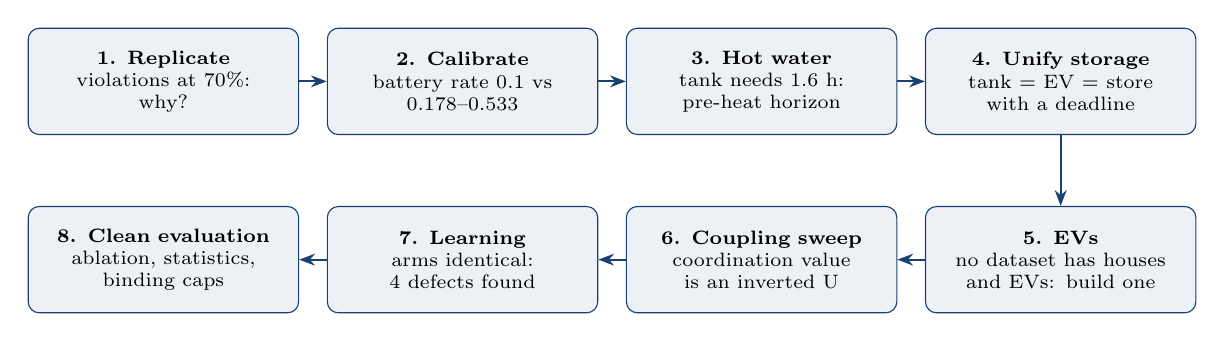
\begin{tikzpicture}[
  node distance=0.35cm and 0.35cm,
  jstep/.style={draw=stemsblue, fill=stemsblue!8, rounded corners, align=center, text width=3.2cm, minimum height=1.35cm, font=\scriptsize},
  arr/.style={-{Stealth[length=2mm]}, thick, stemsblue}]
\node[jstep] (a) {\textbf{1. Replicate}\\violations at 70\%:\\why?};
\node[jstep, right=of a] (b) {\textbf{2. Calibrate}\\battery rate 0.1 vs\\0.178--0.533};
\node[jstep, right=of b] (c) {\textbf{3. Hot water}\\tank needs 1.6 h:\\pre-heat horizon};
\node[jstep, right=of c] (d) {\textbf{4. Unify storage}\\tank = EV = store\\with a deadline};
\node[jstep, below=0.9cm of d] (e) {\textbf{5. EVs}\\no dataset has houses\\and EVs: build one};
\node[jstep, left=of e] (f) {\textbf{6. Coupling sweep}\\coordination value\\is an inverted U};
\node[jstep, left=of f] (g) {\textbf{7. Learning}\\arms identical:\\4 defects found};
\node[jstep, left=of g] (h) {\textbf{8. Clean evaluation}\\ablation, statistics,\\binding caps};
\draw[arr] (a) -- (b); \draw[arr] (b) -- (c); \draw[arr] (c) -- (d);
\draw[arr] (d) -- (e); \draw[arr] (e) -- (f); \draw[arr] (f) -- (g); \draw[arr] (g) -- (h);
\end{tikzpicture}}
\vspace{0.6em}

\small Pattern at every step: \textbf{question} $\rightarrow$ \textbf{measurement} $\rightarrow$ \textbf{mechanism} $\rightarrow$ \textbf{experiment} $\rightarrow$ \textbf{what broke} $\rightarrow$ next question.
\end{frame}

\begin{frame}{Working principles, and the failure behind each}
\small
\begin{tabularx}{\textwidth}{@{}>{\raggedright\arraybackslash}p{0.27\textwidth}X@{}}
\toprule
\textbf{Principle} & \textbf{Why we adopted it} \\
\midrule
Measured, not assumed & A single hard-coded battery rate (0.1) produced most constraint violations. Every rate, capacity and efficiency is now read from the simulator. \\
Fail loud & The original code silently swapped in a mock environment and emitted zero actions when infeasible. Missing data, devices or observations now raise; simulator patches print a banner and are stamped into run metadata. \\
Causal forecasts only & Hot-water demand is forecast from already-observed steps; nothing reads the future. \\
Report negative results & Pre-heating costs money; an inactive mechanism is shown as inactive; each comes with a planned remedy. \\
Regression-check every refactor & The heat-pump-only results are a benchmark in Manal's PhD: every structural change is diffed against the stored results. \\
Verify actuators in every run & The hot-water actuator was inert for months without any error. Each run now proves its actuators respond. \\
\bottomrule
\end{tabularx}
\end{frame}

% =====================================================================
\section{Starting point: replicating STEMS}
% =====================================================================

\begin{frame}{STEMS in one slide}
\begin{columns}[T]
\column{0.55\textwidth}
\textbf{Zhang, Wu, Zinflou and Boulet (2025)}, IEEE Internet of Things Journal, arXiv:2510.14112.
\begin{itemize}
  \item Multi-agent safe RL for building energy management on CityLearn.
  \item \textbf{Spatial} encoder: graph convolution over a building-similarity graph.
  \item \textbf{Temporal} encoder: self-attention over a 24 h history.
  \item Per-building \textbf{actor-critic} (SAC-style) with \textbf{cost critics}.
  \item \textbf{Control barrier function} shield on battery state of charge and power.
  \item \textbf{Lagrangian} pressure so the policy itself learns to be safe.
\end{itemize}
\column{0.45\textwidth}
\begin{block}{Our goal at the start}
Reimplement it faithfully on \textbf{real} data, with every modelling assumption checked against the simulator.
\end{block}
\end{columns}
\end{frame}

\begin{frame}{What we found in the original code}
\begin{columns}[T]
\column{0.5\textwidth}
\begin{alertblock}{Silent fallbacks}
\begin{itemize}
  \item Environment silently swapped to a synthetic \textbf{mock} when the CityLearn import failed.
  \item CBF returned \textbf{all-zero actions} when its optimisation was infeasible.
  \item Trainer used \textbf{raw, unsafe actions} when safe actions were missing.
  \item One \textbf{uniform battery rate} (0.1 per unit action) for every building.
\end{itemize}
\end{alertblock}
\column{0.5\textwidth}
\begin{block}{Consequence}
The one honest run on real data sat at about \textbf{70\% constraint violations}.
\end{block}
\begin{exampleblock}{Response}
\begin{itemize}
  \item Rewrite fail-loud: the mock is reachable only with an explicit flag and a banner.
  \item \texttt{env\_type} and active mechanisms stamped into every result.
  \item Analytic, feasibility-guaranteed projection (never zeros).
  \item Per-building calibration from the simulator.
\end{itemize}
\end{exampleblock}
\end{columns}
\end{frame}

% =====================================================================
\section{The environment}
% =====================================================================

\begin{frame}{The control loop}
\centering
\resizebox{\textwidth}{!}{%
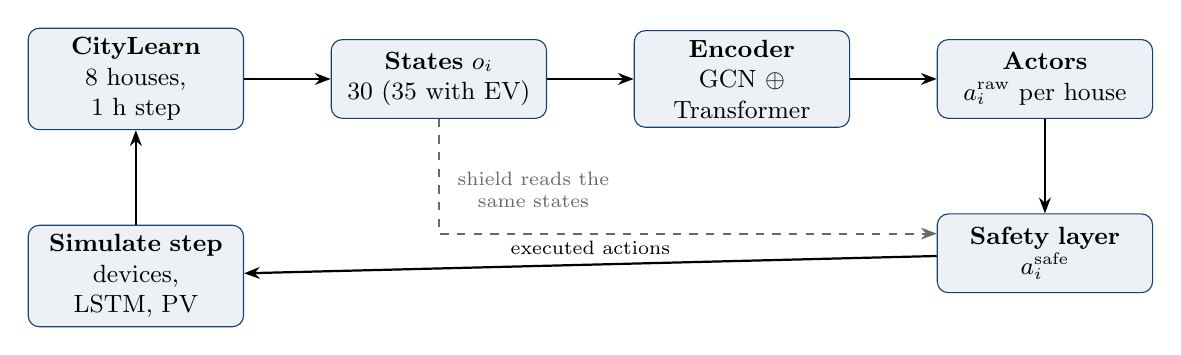
\begin{tikzpicture}[
  box/.style={draw=stemsblue, fill=stemsblue!8, rounded corners, align=center, minimum height=1.0cm, text width=2.5cm, font=\small},
  arr/.style={-{Stealth[length=2mm]}, thick}]
\node[box] (env) {\textbf{CityLearn}\\8 houses, 1 h step};
\node[box, right=1.1cm of env] (obs) {\textbf{States} $o_i$\\30 (35 with EV)};
\node[box, right=1.1cm of obs] (enc) {\textbf{Encoder}\\GCN $\oplus$ Transformer};
\node[box, right=1.1cm of enc] (act) {\textbf{Actors}\\$a_i^{\text{raw}}$ per house};
\node[box, below=1.2cm of act] (shield) {\textbf{Safety layer}\\$a_i^{\text{safe}}$};
\node[box, below=1.2cm of env] (step) {\textbf{Simulate step}\\devices, LSTM, PV};
\draw[arr] (env) -- (obs); \draw[arr] (obs) -- (enc); \draw[arr] (enc) -- (act);
\draw[arr] (act) -- (shield); \draw[arr] (shield) -- node[above, font=\scriptsize]{executed actions} (step);
\draw[arr] (step) -- (env);
\draw[arr, dashed, stemsgray] (obs.south) |- ($(shield.west)+(0,0.25)$);
\node[font=\scriptsize, stemsgray, align=center] at ($(obs.south)+(1.2,-0.9)$) {shield reads the\\same states};
\end{tikzpicture}}
\vspace{0.5em}

\small Every hour: observe $\rightarrow$ encode $\rightarrow$ propose $\rightarrow$ project onto the safe set $\rightarrow$ simulate. Rewards, costs and KPIs are computed from the \textbf{observed} next state, never from the shield's internal model.
\end{frame}

\begin{frame}{Dataset and scenario}
\centering
\small
\begin{tabular}{@{}ll@{}}
\toprule
Simulator & CityLearn 2.6.0b1 (Gymnasium API) \\
Building data & NREL ResStock, release \texttt{amy2018-2021}; calendar matches 2018 \\
Location & Travis County, Texas (cooling-dominated) \\
Buildings & 8 simulated out of 100 candidates; decentralised control \\
Horizon & 8760 hourly steps (one year) \\
Devices per house & heating heat pump, cooling heat pump, electric hot-water heater, \\
 & hot-water tank, battery, rooftop PV \\
Building type & \texttt{LSTMDynamicsBuilding} (indoor temperature from an LSTM) \\
Device sizing & autosized by CityLearn \textbf{at construction}, from the simulation period \\
Active observations & 45; STEMS selects 28 by name, 30 with heat-pump features \\
Actions & \texttt{[dhw\_storage, electrical\_storage, cooling\_or\_heating\_device]} \\
Prices, carbon & files borrowed from the CityLearn 2022 challenge (California) \\
\bottomrule
\end{tabular}
\end{frame}

\begin{frame}{Devices and their sizes (full-year autosizing, all 100 candidates)}
\begin{columns}[T]
\column{0.56\textwidth}
\footnotesize
\begin{tabular}{@{}lll@{}}
\toprule
Device & Model & Size range \\
\midrule
Heating & heat pump & 2.04--21.10 kW \\
Cooling & heat pump & 1.10--12.53 kW \\
Hot-water heater & electric heater & 3.94--17.32 kW \\
Hot-water tank & storage tank & 0--12.48 kWh \\
Battery & battery & 3.30--24.50 kWh \\
 & & 1.28--7.07 kW \\
PV & PySAM PVWatts & 3.82--26.80 kW \\
\bottomrule
\end{tabular}
\column{0.42\textwidth}
\begin{alertblock}{Not every house is equipped}
\begin{itemize}
  \item \textbf{61 of 100} candidates have \textbf{no hot-water tank}.
  \item \textbf{39 of 100} have every device.
  \item The reference eight are all fully equipped.
\end{itemize}
\end{alertblock}
\small Our wrapper reported missing tanks as capacity 1.0: a silent fallback, \tagtodo. Building subsets will be drawn from the 39 fully equipped houses (the sampler currently draws from all 100).
\end{columns}
\end{frame}

\begin{frame}{Device physics: storage (battery and hot-water tank)}
Both devices share CityLearn's storage model. For requested energy $e$ (positive = charge), capacity $C$, round-trip efficiency $\eta$, standby loss $\lambda$:
\begin{align*}
\SOC^{\text{init}} &= \max\big(0,\ \SOC_{t-1}\, C\,(1-\lambda)\big)\\[2pt]
\SOC_t &= \frac{1}{C}
\begin{cases}
\min\big(\SOC^{\text{init}} + e\sqrt{\eta},\ C\big) & e \ge 0 \quad\text{(charge)}\\[2pt]
\max\big(0,\ \SOC^{\text{init}} + e/\sqrt{\eta}\big) & e < 0 \quad\text{(discharge)}
\end{cases}
\end{align*}
\begin{columns}[T]
\column{0.5\textwidth}
\textbf{Battery}: $e = a\,P_{\text{nom}}\,\Delta t$. So the state of charge moves by about
\[
\rho_i = P_{\text{nom},i}/C_i \quad\text{per unit action.}
\]
\column{0.5\textwidth}
\textbf{Hot-water tank}: $e = a\,C$, clipped to what the heater can deliver in one hour (next slides).
\end{columns}
\vspace{0.4em}
\begin{block}{Why this matters}
$\rho_i$ is the quantity the safety barrier needs. Getting it wrong by a factor of 2--5 was the main source of violations.
\end{block}
\end{frame}

\begin{frame}{Device physics: heat pump}
\small
Carnot coefficient of performance, efficiency $\eta$, supply temperature $T_{\text{tgt}}$ (measured: $\eta \in [0.21, 0.29]$ cooling, $[0.20, 0.28]$ heating; supply 7.2--9.8 and 45.2--48.8\,$^\circ$C):
\[
\mathrm{CoP}_{\text{heat}}(T_{\text{out}}) = \eta\,\frac{T^{\text{heat}}_{\text{tgt}} + 273.15}{T^{\text{heat}}_{\text{tgt}} - T_{\text{out}}},
\qquad
\mathrm{CoP}_{\text{cool}}(T_{\text{out}}) = \eta\,\frac{T^{\text{cool}}_{\text{tgt}} + 273.15}{T_{\text{out}} - T^{\text{cool}}_{\text{tgt}}}
\]
\[
P_{\text{out}} = \min\big(|a|\,P_{\text{nom}},\ P_{\text{nom}}\big)\cdot \mathrm{CoP},
\qquad
P_{\text{in}} = P_{\text{out}} / \mathrm{CoP}, \qquad \mathrm{CoP} \le 20
\]
\begin{columns}[T]
\column{0.53\textwidth}
\begin{alertblock}{The sign of the action picks the mode}
CityLearn splits one action into two devices,
$a^{\text{cool}} = |\min(a, 0)|$ and $a^{\text{heat}} = \max(a, 0)$: $a<0$ cools, $a>0$ heats, each against its own nominal power. The \texttt{hvac\_mode} gate can disable a mode, but it equals 3 (both allowed) at \textbf{every hour of all eight houses}.
\end{alertblock}
\column{0.47\textwidth}
\begin{block}{Consequences}
\begin{itemize}
  \item Comfort needs a \textbf{dual set-point deadband}: the agent may heat or cool at any hour.
  \item Anything that assumes the mode --- our CoP guard reads it off the weather, the rule-based baseline sends $+0.2$ ``for cooling'' --- is wrong by construction (see the defects).
\end{itemize}
\end{block}
\end{columns}
\end{frame}

\begin{frame}{Device physics: hot water, and the lead time}
Electric heater: $P_{\text{out}} = \min(|a|P_{\text{nom}}, P_{\text{nom}})\,\eta$, $\eta \approx 0.9$--$0.99$. The tank is charged by $e = a\,C$, clipped to the heater's hourly output, so the state-of-charge gain per step is
\[
\boxed{\ \rho^{\text{dhw}}_i = \min\!\Big(c_i,\ \frac{P_{\text{nom},i}\,\eta_i}{C_i}\Big), \qquad \tau_i = \frac{1}{\rho^{\text{dhw}}_i}\ \text{hours to fill an empty tank}\ }
\]
with $c_i$ CityLearn's per-building action bound.
\vspace{0.3em}
\begin{columns}[T]
\column{0.5\textwidth}
\begin{exampleblock}{Measured on the reference eight}
$\rho^{\text{dhw}} \in [0.52, 0.85]$, \quad $\tau \in [1.17, 1.92]$\,h, \quad mean $1.60$\,h.\\[2pt]
Validated: one maximum-charge step from empty lands within 15\% of $\rho^{\text{dhw}}_i$ in every house.
\end{exampleblock}
\column{0.5\textwidth}
\begin{block}{The idea this created}
Hot water cannot be made on demand. A controller that reacts \textbf{after} seeing demand is structurally too late: it must \textbf{pre-heat}, with a horizon at least as long as $\tau$.
\end{block}
\end{columns}
\end{frame}

\begin{frame}{How net consumption, cost and emissions are computed}
CityLearn, every step, for building $i$ (PV generation is stored as a \textbf{negative} value):
\[
e_{i,t} = E^{\text{cool}}_{i,t} + E^{\text{heat}}_{i,t} + E^{\text{dhw}}_{i,t} + E^{\text{nsl}}_{i,t} + E^{\text{batt}}_{i,t} + E^{\text{EV}}_{i,t} + E^{\text{wm}}_{i,t} + \mathrm{PV}_{i,t}
\]
\begin{columns}[T]
\column{0.5\textwidth}
\textbf{CityLearn's own bookkeeping}
\begin{align*}
\text{cost}_{i,t} &= e_{i,t}\, v_t \quad(\text{can be negative})\\
\text{emission}_{i,t} &= \max\big(0,\ e_{i,t}\,\kappa_t\big)
\end{align*}
\column{0.5\textwidth}
\textbf{Our KPIs}
\begin{align*}
\text{cost} &= \textstyle\sum_{t,i} \max(e_{i,t},0)\, v_t \quad(\text{imports only})\\
\text{emission} &= \textstyle\sum_{t,i} \max(e_{i,t},0)\, \kappa_t
\end{align*}
\end{columns}
\vspace{0.3em}
\small $E^{\text{cool}}, E^{\text{heat}}, E^{\text{dhw}}$: device electricity; $E^{\text{nsl}}$: non-shiftable load; $E^{\text{batt}}$: battery (charge $+$, discharge $-$); $E^{\text{EV}}$: chargers; $E^{\text{wm}}$: washing machines (none here); $v_t$: price; $\kappa_t$: carbon intensity.
\end{frame}

\begin{frame}{How indoor temperature is simulated}
\begin{columns}[T]
\column{0.55\textwidth}
\textbf{\texttt{LSTMDynamicsBuilding}}: every house has its own trained LSTM surrogate.
\begin{itemize}
  \item 2 layers, hidden size 8, look-back 13\,h, one \texttt{.pth} file per house.
  \item \textbf{13 min-max normalised inputs}: $\sin/\cos$ of month, day type and hour; cooling demand; heating demand; direct and diffuse irradiance; outdoor temperature; occupant count; and the \textbf{previous indoor temperature}.
  \item Output: indoor dry-bulb temperature for the current step, un-normalised and written back into the state.
  \item Warm-up: the heat pump is only controllable once the look-back is filled.
\end{itemize}
\column{0.45\textwidth}
\begin{block}{Why it matters}
Comfort responds to HVAC actions through a \textbf{learned model}, not EnergyPlus itself. Comfort results are only as good as that surrogate.
\end{block}
\begin{block}{Consequence for us}
Indoor temperature is a \textbf{simulated state}, not a data column, whenever the heat pump is controlled.
\end{block}
\end{columns}
\end{frame}

% =====================================================================
\section{The states: what the agent sees and where it comes from}
% =====================================================================

\begin{frame}{Structure of the observation vector}
For each building $i$:
\[
o_i = \Big[\ \underbrace{x^{\text{base}}_i}_{28}\ ,\ \underbrace{x^{\text{hp}}_i}_{2\ (\text{heat-pump mode})}\ ,\ \underbrace{x^{\text{ev}}_{i,1},\ \dots,\ x^{\text{ev}}_{i,K}}_{5 \text{ per charger slot}}\ \Big]
\]
\begin{columns}[T]
\column{0.5\textwidth}
\small
\begin{tabular}{@{}lr@{}}
\toprule
Environment & dimension \\
\midrule
Travis 8 houses & 28 \\
Travis, heat-pump mode & 30 \\
Travis + EVs (merged) & 35 \\
EV challenge, 17 houses & 38 \\
\bottomrule
\end{tabular}
\column{0.5\textwidth}
\begin{block}{Selected by name}
Features are mapped from CityLearn's names, not positions, so the selection is auditable and survives schema reordering. A missing feature raises instead of being zero-filled.
\end{block}
\end{columns}
\end{frame}

\begin{frame}{The 30 base states (1/2)}
\scriptsize
\begin{tabularx}{\textwidth}{@{}rl>{\raggedright\arraybackslash}X>{\raggedright\arraybackslash}p{4.2cm}@{}}
\toprule
\# & Feature & Meaning, unit & Where it comes from \\
\midrule
0 & \texttt{day\_type} & day of week, 1 = Monday \dots\ 7 = Sunday & building CSV (calendar) \\
1 & \texttt{hour} & hour of day, \textbf{1--24} & building CSV (calendar) \\
2 & \texttt{outdoor\_dry\_bulb\_temperature} & $^\circ$C & \texttt{weather.csv} (actual meteorological year) \\
3--5 & \quad \texttt{\_predicted\_1,2,3} & forecast at \textbf{+6, +12, +24 h} & \texttt{weather.csv} (verified by lag analysis) \\
6 & \texttt{diffuse\_solar\_irradiance} & W/m$^2$ & \texttt{weather.csv} \\
7--9 & \quad \texttt{\_predicted\_1,2,3} & +6, +12, +24 h & \texttt{weather.csv} \\
10 & \texttt{direct\_solar\_irradiance} & W/m$^2$ & \texttt{weather.csv} \\
11--13 & \quad \texttt{\_predicted\_1,2,3} & +6, +12, +24 h & \texttt{weather.csv} \\
14 & \texttt{carbon\_intensity} & kg CO$_2$/kWh & \texttt{carbon\_intensity.csv} (2022 challenge) \\
15 & \texttt{indoor\_dry\_bulb\_temperature} & $^\circ$C & \textbf{simulated}: per-house LSTM \\
16 & \texttt{non\_shiftable\_load} & kWh & building CSV (ResStock end use) \\
17 & \texttt{solar\_generation} & kWh & PV size $\times$ PySAM per-kW series \\
\bottomrule
\end{tabularx}
\end{frame}

\begin{frame}{The 30 base states (2/2)}
\scriptsize
\begin{tabularx}{\textwidth}{@{}rl>{\raggedright\arraybackslash}X>{\raggedright\arraybackslash}p{4.2cm}@{}}
\toprule
\# & Feature & Meaning, unit & Where it comes from \\
\midrule
18 & \texttt{dhw\_storage\_soc} & tank state of charge $\in[0,1]$ & \textbf{device state} (tank model) \\
19 & \texttt{electrical\_storage\_soc} & battery state of charge $\in[0,1]$ & \textbf{device state} (battery model) \\
20 & \texttt{net\_electricity\_consumption} & kWh (negative = export) & \textbf{computed} each step (net load formula) \\
21 & \texttt{electricity\_pricing} & \$/kWh & \texttt{pricing.csv} (2022 challenge) \\
22--23 & \quad \texttt{\_predicted\_1,2} & +6, +12 h, \textbf{exact} & \texttt{pricing.csv} (perfect foresight) \\
24 & \texttt{cooling\_demand} & kWh thermal & building CSV (EnergyPlus load) \\
25 & \texttt{dhw\_demand} & kWh thermal, \textbf{current hour only} & building CSV \\
26 & \texttt{occupant\_count} & persons & building CSV \\
27 & \texttt{indoor\_..\_cooling\_set\_point} & $^\circ$C & building CSV \\
\midrule
28 & \texttt{indoor\_..\_heating\_set\_point} & $^\circ$C (heat-pump mode) & building CSV \\
29 & \texttt{heating\_electricity\_consumption} & kWh (heat-pump mode) & \textbf{computed}: heat-pump draw \\
\bottomrule
\end{tabularx}
\vspace{0.3em}

\small \texttt{heating\_demand} exists in the building CSV but is not an active observation, so the heating electricity draw is used as the heating-load signal.
\end{frame}

\begin{frame}{Five kinds of state, five different origins}
\centering
\resizebox{\textwidth}{!}{%
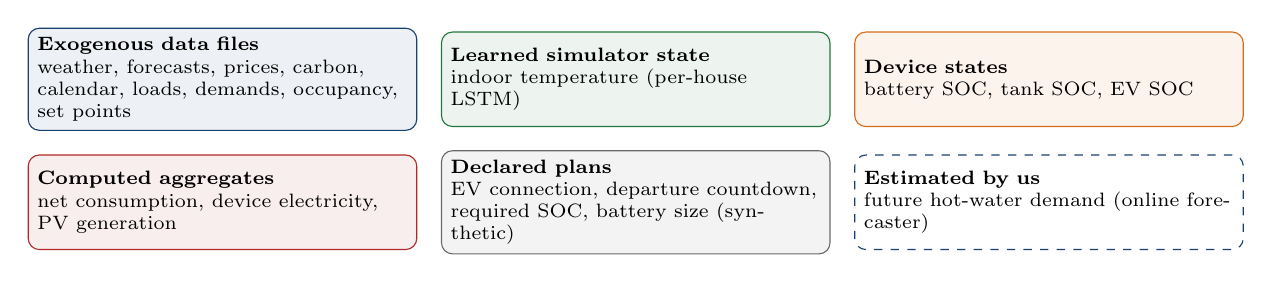
\begin{tikzpicture}[
  cat/.style={draw, rounded corners, align=left, text width=4.7cm, minimum height=1.2cm, font=\scriptsize},
  node distance=0.3cm]
\node[cat, draw=stemsblue, fill=stemsblue!8] (a) {\textbf{Exogenous data files}\\weather, forecasts, prices, carbon, calendar, loads, demands, occupancy, set points};
\node[cat, draw=stemsgreen, fill=stemsgreen!8, right=of a] (b) {\textbf{Learned simulator state}\\indoor temperature (per-house LSTM)};
\node[cat, draw=stemsorange, fill=stemsorange!8, right=of b] (c) {\textbf{Device states}\\battery SOC, tank SOC, EV SOC};
\node[cat, draw=stemsred, fill=stemsred!8, below=of a] (d) {\textbf{Computed aggregates}\\net consumption, device electricity, PV generation};
\node[cat, draw=stemsgray, fill=stemsgray!8, right=of d] (e) {\textbf{Declared plans}\\EV connection, departure countdown, required SOC, battery size (synthetic)};
\node[cat, draw=stemsblue, dashed, right=of e] (f) {\textbf{Estimated by us}\\future hot-water demand (online forecaster)};
\end{tikzpicture}}
\vspace{0.6em}

\small \textbf{Only the actions change} device states, computed aggregates and the LSTM temperature. Everything in the blue box is fixed data: the agent cannot influence weather, prices or demand, only when energy is drawn and stored.
\end{frame}

\begin{frame}{Calendar conventions: verified against real dates}
\begin{columns}[T]
\column{0.5\textwidth}
\textbf{Hour}\\[2pt]
\small
\begin{tabular}{@{}lllll@{}}
\toprule
step & 0 & 1 & 2 & 3 \\
hour & 1 & 2 & 3 & 4 \\
\midrule
step & 22 & 23 & 24 & 25 \\
hour & 23 & 24 & 1 & 2 \\
\bottomrule
\end{tabular}\\[4pt]
\normalsize $\Rightarrow$ \texttt{hour} $\in \{1,\dots,24\}$, where 1 is 00:00--01:00.
\column{0.5\textwidth}
\textbf{Day type}\\[2pt]
\small
\begin{tabular}{@{}lll@{}}
\toprule
step & date (2018) & \texttt{day\_type} \\
\midrule
0 & 1 January, Monday & 1 \\
672 & 29 January, Monday & 1 \\
4344 & 1 July, Sunday & 7 \\
\bottomrule
\end{tabular}\\[4pt]
\normalsize $\Rightarrow$ 1 = Monday \dots\ 7 = Sunday.
\end{columns}
\vspace{0.6em}
\begin{alertblock}{Two defects found while preparing this presentation}
\begin{itemize}
  \item Our hot-water forecaster treats \texttt{day\_type} $\in\{1,7,8\}$ as weekend: \textbf{Monday} counted as weekend, \textbf{Saturday} as weekday.
  \item It clips \texttt{hour} to 0--23: hours 23 and 24 share a slot and slot 0 never fills.
\end{itemize}
Both are \tagtodo; the pre-heating results (E4, E5) use the forecaster and will be recomputed.
\end{alertblock}
\end{frame}

\begin{frame}{How the forecasts are generated: a lag analysis of the data}
\small
For each \texttt{\_predicted\_k} column we searched the lag $\ell \in \{0,\dots,48\}$ that minimises $\frac{1}{T}\sum_t |\hat x^{(k)}_t - x_{t+\ell}|$.
\vspace{0.3em}
\centering
\begin{tabular}{@{}lccccc@{}}
\toprule
Variable & \texttt{predicted\_1} & \texttt{predicted\_2} & \texttt{predicted\_3} & signal mean abs.\ dev. \\
\midrule
Outdoor temperature & +6 h, MAE 0.15\,$^\circ$C & +12 h, 0.33 & +24 h, 0.69 & 7.59\,$^\circ$C \\
Direct irradiance & +6 h, 2.69 W/m$^2$ & +12 h, 5.36 & +24 h, 10.68 & 273.5 W/m$^2$ \\
Diffuse irradiance & +6 h, 0.81 W/m$^2$ & +12 h, 1.60 & +24 h, 3.23 & 70.4 W/m$^2$ \\
Relative humidity & +6 h, 0.83\,\% & +12 h, 1.65 & +24 h, 3.28 & 18.1\,\% \\
Electricity price & +6 h, \textbf{0.0000} & +12 h, \textbf{0.0000} & +24 h, \textbf{0.0000} & 0.095 \$/kWh \\
\bottomrule
\end{tabular}
\vspace{0.5em}
\begin{columns}[T]
\column{0.5\textwidth}
\begin{block}{Reading}
Weather forecasts are the future actuals plus \textbf{small noise that grows with horizon}. Price forecasts are \textbf{perfect foresight}.
\end{block}
\column{0.5\textwidth}
\begin{block}{Runtime noise}
CityLearn can add Gaussian noise (\texttt{noise\_std}) to weather actuals and forecasts; its default is 0, so nothing is added at runtime.
\end{block}
\end{columns}
\end{frame}

\begin{frame}{What the forecast horizons mean for control}
\begin{columns}[T]
\column{0.5\textwidth}
\begin{alertblock}{A third defect}
Our thermal code assumed the three predictions were \textbf{+1, +2, +3 h}. They are \textbf{+6, +12, +24 h}. Affected, and \tagtodo:
\begin{itemize}
  \item the temperature uplift in the hot-water forecaster,
  \item the cold-front term (it looks 6--24 h ahead, not 1--3 h),
  \item the stress-test front, which ramped per forecast, not per hour.
\end{itemize}
\end{alertblock}
\column{0.5\textwidth}
\begin{block}{Horizons against lead times}
\small
\begin{tabular}{@{}ll@{}}
\toprule
Hot-water tank fill time & 1.6 h \\
EV fill time & 5.7--7.4 h \\
Weather / price forecasts & 6, 12, 24 h \\
\bottomrule
\end{tabular}
\end{block}
\begin{block}{Implications}
\begin{itemize}
  \item Forecasts reach beyond the tank's lead time and cover the EV's.
  \item Perfect price foresight makes price-aware results \textbf{optimistic}: the forecast-error experiment is needed.
\end{itemize}
\end{block}
\end{columns}
\end{frame}

\begin{frame}{Prices and carbon intensity}
\begin{columns}[T]
\column{0.5\textwidth}
\begin{alertblock}{Borrowed data}
The Travis schema points to \texttt{pricing.csv} and \texttt{carbon\_intensity.csv} from the \textbf{CityLearn 2022 challenge (California)}. They are not a Texas tariff.
\end{alertblock}
\small
\begin{tabular}{@{}ll@{}}
\toprule
Price levels & 0.21, 0.22, 0.40, 0.50, 0.54 \$/kWh \\
Structure & time-of-use \\
Carbon intensity & 0.070--0.282 kg CO$_2$/kWh \\
\bottomrule
\end{tabular}
\column{0.5\textwidth}
\begin{block}{How we use them}
\begin{itemize}
  \item Economic reward term: $-\mu\, v_t\, e_{i,t}$.
  \item Cost and emission KPIs (imports only).
  \item Price forecasts feed the policy (+6, +12 h).
\end{itemize}
\end{block}
\begin{block}{Caveat for claims}
Any cost number is relative to this tariff; the Thermia and Nordic scenarios need their own spot prices.
\end{block}
\end{columns}
\end{frame}

\begin{frame}{What the agent cannot observe, and how we handle it}
\small
\begin{tabularx}{\textwidth}{@{}>{\raggedright\arraybackslash}p{3.3cm}>{\raggedright\arraybackslash}X>{\raggedright\arraybackslash}p{4.8cm}@{}}
\toprule
Missing information & Why it matters & What we do \\
\midrule
Future hot-water demand & Tank needs 1.6 h to fill; demand is only visible in the current hour & Causal online climatology per house, hour and day type (next slide) \\
Heating demand & Not an active observation & Heating electricity draw as proxy \\
Future EV arrivals & Deadlines appear only on arrival & Barrier acts on connected vehicles; incoming-vehicle signals exist but are not in the STEMS subset \\
Tank temperature & Legionella needs 60\,$^\circ$C; CityLearn tanks store energy only & Temperature proxy or tank extension (planned) \\
Forecast uncertainty & Data forecasts are near-perfect & Controlled error injection (planned experiment) \\
\bottomrule
\end{tabularx}
\end{frame}

\begin{frame}{Estimating future hot-water demand (causal, online)}
For house $i$, hour slot $h$ and day class $w$ (weekday or weekend), an exponentially weighted mean over \textbf{already observed} steps:
\[
m_{i,h,w} \leftarrow m_{i,h,w} + \alpha\,\big(d_{i,t} - m_{i,h,w}\big), \qquad \alpha = 0.2
\]
Forecast over the pre-heat horizon $L$, with a cold-weather uplift $g$:
\[
\hat D_i(L) = \sum_{k=1}^{L} m_{i,\,(h+k) \bmod 24,\,w}\ \big(1 + g\,\mathrm{relu}(\bar T - \hat T_{t+k})\big), \qquad g = 0.02
\]
\begin{columns}[T]
\column{0.5\textwidth}
\begin{block}{Properties}
\begin{itemize}
  \item No look-ahead: only past steps enter $m$.
  \item Warm-up (first 24 steps): $\hat D_i(L) = L\cdot d_{i,t}$, never below current demand.
  \item Learns on site, per installation, without data leaving the house.
\end{itemize}
\end{block}
\column{0.5\textwidth}
\begin{alertblock}{Corrections pending}
\begin{itemize}
  \item Slot: $h = \texttt{hour} - 1$ (data are 1--24).
  \item Weekend: \texttt{day\_type} $\in \{6,7,8\}$.
  \item $\hat T_{t+k}$ must use the forecast whose horizon matches (6/12/24 h).
\end{itemize}
\end{alertblock}
\end{columns}
\end{frame}

\begin{frame}{EV states and how the schedules are generated}
\begin{columns}[T]
\column{0.5\textwidth}
\textbf{Per charger slot (5 states)}
\small
\begin{tabular}{@{}ll@{}}
\toprule
\texttt{connected\_state} & 1 if a car is plugged in \\
\texttt{departure\_time} & countdown in \textbf{steps} \\
\texttt{required\_soc\_departure} & fraction (CSV stores \%) \\
\texttt{soc} & current state of charge \\
\texttt{battery\_capacity} & kWh of the car present \\
\bottomrule
\end{tabular}\\[4pt]
\normalsize
\textbf{Hardware (6 of 8 houses)}: chargers alternate 11 / 7.4 kW, $\eta = 0.95$, 7.2 kW discharge (V2G capable); batteries 60, 40, 75, 52, 60, 40 kWh.
\column{0.5\textwidth}
\begin{alertblock}{Synthetic schedules (ResStock has no vehicles)}
\small
\begin{tabular}{@{}lll@{}}
\toprule
 & weekday & weekend \\
\midrule
stays home & 12\,\% & 45\,\% \\
departs & $\mathcal N(7.5, 0.8)$ h & $\mathcal N(9.5, 1.5)$ h \\
returns & $\mathcal N(17.5, 1.2)$ h & $\mathcal N(15.5, 2.0)$ h \\
\bottomrule
\end{tabular}
\begin{itemize}
  \item Required SOC $\sim \mathcal U(0.70, 0.90)$.
  \item Arrival SOC $\sim \mathcal U(0.25,0.55) - 0.01(\text{hours away} - 8)$, clipped to $[0.10, 0.60]$.
  \item Countdown reaches 0 \textbf{while still parked}: the departure hour is a last charging opportunity.
\end{itemize}
\end{alertblock}
\end{columns}
\end{frame}

\begin{frame}{Heterogeneous houses: one shape for the graph network}
\begin{columns}[T]
\column{0.5\textwidth}
\textbf{The problem.} In the EV challenge dataset houses differ: native actions 1--3, observations 28--42, charger ids embedded in feature names. The GCN stacks houses into one matrix, so every house needs the same vector.

\vspace{0.4em}
\textbf{Canonical padded layout}
\begin{itemize}
  \item States = base features + $5K$ EV slots; a house with fewer bays is zero-padded.
  \item Actions = canonical order restricted to devices some house owns.
  \item Per-house index map; presence mask $M \in \{0,1\}^{B\times A}$.
\end{itemize}
\column{0.5\textwidth}
\begin{block}{Two design choices}
\begin{itemize}
  \item A padded slot reports \texttt{connected\_state} $=0$, which the EV barrier already reads as ``no vehicle'': one code path, no special case.
  \item Actions for absent devices are \textbf{dropped} before CityLearn, not sent as zeros.
\end{itemize}
\end{block}
\begin{exampleblock}{Verified}
17 heterogeneous houses $\rightarrow$ one $(38,)$ vector; on Travis every map is the identity, so earlier results are unchanged.
\end{exampleblock}
\end{columns}
\end{frame}

\begin{frame}{Normalisation and temporal context}
\begin{columns}[T]
\column{0.5\textwidth}
\textbf{Running normalisation}\\[2pt]
Each feature $j$ is standardised with a running mean and variance updated from every training episode:
\[
\hat o_{i,j} = \frac{o_{i,j} - \mu_j}{\sqrt{\sigma^2_j + \epsilon}}
\]
The normaliser is saved with the model and reused unchanged at evaluation.
\column{0.5\textwidth}
\textbf{History window}\\[2pt]
Each house keeps its last $T = 24$ hourly observations,
\[
H_{i,t} = \big[\hat o_{i,t-23}, \dots, \hat o_{i,t}\big] \in \R^{24 \times d},
\]
which the temporal encoder attends over. The spatial encoder sees the current $\hat o_{i,t}$ of all houses.
\end{columns}
\vspace{0.6em}
\begin{block}{Why both}
Weather, prices and demand have daily structure (temporal); houses on one feeder share weather and constraints (spatial).
\end{block}
\end{frame}

% =====================================================================
\section{The learning architecture}
% =====================================================================

\begin{frame}{From states to actions}
\centering
\resizebox{\textwidth}{!}{%
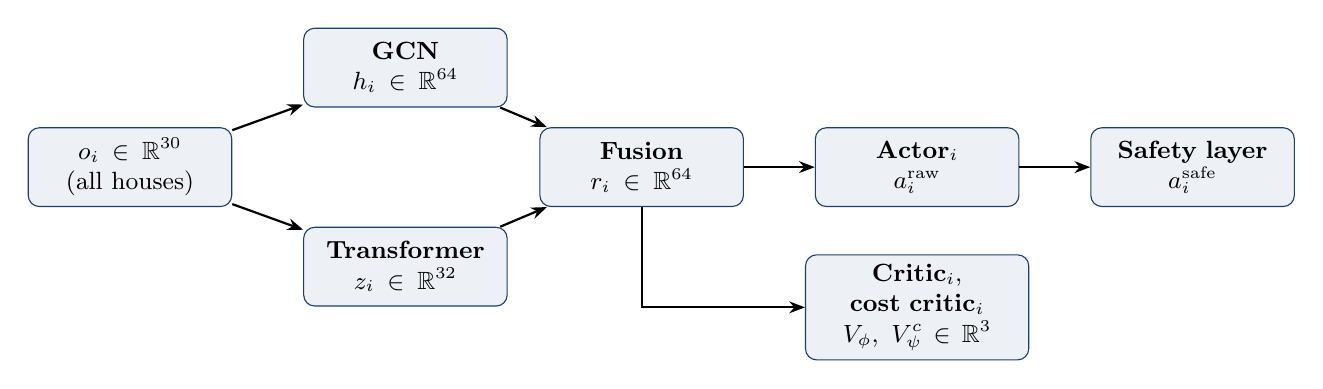
\begin{tikzpicture}[
  box/.style={draw=stemsblue, fill=stemsblue!8, rounded corners, align=center, minimum height=1.0cm, text width=2.35cm, font=\small},
  arr/.style={-{Stealth[length=2mm]}, thick}]
\node[box] (o) {$o_i \in \R^{30}$\\(all houses)};
\node[box, above right=0.25cm and 0.9cm of o] (g) {\textbf{GCN}\\$h_i \in \R^{64}$};
\node[box, below right=0.25cm and 0.9cm of o] (t) {\textbf{Transformer}\\$z_i \in \R^{32}$};
\node[box, right=3.9cm of o] (f) {\textbf{Fusion}\\$r_i \in \R^{64}$};
\node[box, right=0.9cm of f] (a) {\textbf{Actor}$_i$\\$a_i^{\text{raw}}$};
\node[box, right=0.9cm of a] (s) {\textbf{Safety layer}\\$a_i^{\text{safe}}$};
\node[box, below=0.6cm of a, text width=2.6cm] (c) {\textbf{Critic}$_i$, \textbf{cost critic}$_i$\\$V_\phi,\ V^c_\psi \in \R^3$};
\draw[arr] (o) -- (g); \draw[arr] (o) -- (t); \draw[arr] (g) -- (f); \draw[arr] (t) -- (f);
\draw[arr] (f) -- (a); \draw[arr] (a) -- (s); \draw[arr] (f) |- (c);
\end{tikzpicture}}
\vspace{0.6em}

\small The encoder is \textbf{shared} by all houses; each house has its \textbf{own} actor, value critic and three-headed cost critic (battery SOC, house power, grid power).
\end{frame}

\begin{frame}{Building-similarity graph}
\[
w_{ij} = \alpha\,\exp\!\Big(-\frac{d_{ij}^2}{2\sigma_d^2}\Big) + \beta\,\exp\!\Big(-\frac{\|f_i - f_j\|^2}{2\sigma_f^2}\Big),
\qquad w_{ii} = 0
\]
\begin{columns}[T]
\column{0.5\textwidth}
\begin{itemize}
  \item $d_{ij}$: geographic distance (latitude, longitude).
  \item $f_i$: normalised battery capacity and floor area.
  \item $\alpha = \beta = 0.5$, \ $\sigma_d = \sigma_f = 1$.
\end{itemize}
\column{0.5\textwidth}
\begin{alertblock}{Finding}
On the eight co-located Travis houses every off-diagonal weight is \textbf{0.80--1.00}. The graph is near-complete and near-uniform, so message passing is close to \textbf{averaging over all houses}.
\end{alertblock}
\end{columns}
\vspace{0.4em}
\begin{block}{Consequence}
Removing the graph (``decentralised'') and keeping it (``coordinated'') moved the raw actions by only 0.001--0.008. A coordination benefit needs either a sharper graph or a constraint that couples the houses.
\end{block}
\end{frame}

\begin{frame}{Spatial encoder: graph convolution}
Three layers, width 64, $\sigma = \mathrm{ReLU}$, adjacency with self-loops $\hat A = A + I$:
\[
H^{(l+1)} = \sigma\Big(\hat D^{-1/2}\,\hat A\,\hat D^{-1/2}\, H^{(l)}\, W^{(l)}\Big),
\qquad \hat D_{ii} = \sum_j \hat A_{ij},
\qquad H^{(0)} = \big[\hat o_1, \dots, \hat o_B\big]^\top
\]
\vspace{0.3em}
\begin{columns}[T]
\column{0.5\textwidth}
\begin{block}{Reading}
Each house's representation mixes its own state with its neighbours', weighted by similarity.
\end{block}
\column{0.5\textwidth}
\begin{block}{The decentralised ablation in one line}
Set $A = 0$. Then $\hat A = I$ and $h_i$ depends only on house $i$: same parameters, same optimiser, one knob.
\end{block}
\end{columns}
\end{frame}

\begin{frame}{Temporal encoder: self-attention over 24 hours}
Four heads, 32-dimensional embedding, fixed sinusoidal positional encodings, window $T = 24$:
\[
e_{\tau,\tau'} = \frac{Q_\tau K_{\tau'}^\top}{\sqrt{d_k}},
\qquad
z_{i,t} = \mathrm{LayerNorm}\Big(x_{i,t} + \sum_{\tau'} \mathrm{softmax}_{\tau'}\big(e_{t,\tau'}\big)\, V_{\tau'}\Big)
\]
with $Q, K, V$ linear projections of the embedded history $H_{i,t}$.
\vspace{0.5em}
\begin{block}{What it can learn}
Daily patterns in load, prices and occupancy, and which past hours predict the next decision, without a hand-written feature for each.
\end{block}
\end{frame}

\begin{frame}{Fusion, actors and critics}
\[
r_i = W_s\, h_i + W_t\, z_i + b \in \R^{64}
\]
\small
\begin{columns}[T]
\column{0.52\textwidth}
\textbf{Squashed-Gaussian actor (per house)}
\begin{align*}
u &\sim \mathcal N\big(\mu_\theta(r_i),\ \sigma_\theta(r_i)^2\big), \quad a = \tanh(u)\\
\log \pi_\theta(a\mid r_i) &= \log \mathcal N(u;\mu,\sigma^2)\\
 &\quad - \textstyle\sum_d \log\big(1 - \tanh^2(u_d) + \epsilon\big)
\end{align*}
\column{0.48\textwidth}
\textbf{Critics (per house)}
\begin{align*}
V_\phi(r_i) &\in \R \quad\text{value}\\
V^c_\psi(r_i) &\in \R^3 \quad\text{expected cost of}\\
&\qquad\text{SOC, house power, grid power}
\end{align*}
\end{columns}
\vspace{0.4em}
\small Hidden width 128, learning rate $3\cdot 10^{-4}$, discount $\gamma = 0.99$, target critics with soft update $\tau = 0.005$, entropy temperature auto-tuned to target $-|\mathcal A|$.
\end{frame}

\begin{frame}{Reward: four terms}
\begin{align*}
r^{\text{econ}}_i &= -\mu\, v_t\, e_i\\
r^{\text{stab}}_i &= \alpha_g\Big(1 - \tfrac{E_{\text{grid}}}{P_{\text{grid,max}}}\Big)^2 + \alpha_b\Big(1 - \tfrac{|e_i|}{P_{\text{bldg,max}}}\Big) - \beta_r\,\tfrac{|e_i - e_i^{\text{prev}}|}{P_{\text{bldg,max}}}\\
r^{\text{comfort}}_i &= -\lambda_c\, d(T^{\text{in}}_i)^2,
\qquad
d(T) = \begin{cases} T - T^{\text{cool}} & T > T^{\text{cool}}\\ T^{\text{heat}} - T & T < T^{\text{heat}}\\ 0 & \text{inside the deadband}\end{cases}\\
r^{\text{renew}}_i &= \xi\,\min\Big(\tfrac{\text{solar}_i}{\max(\text{load}_i,\epsilon)},\ 1\Big)
\end{align*}
\small $E_{\text{grid}} = \sum_i \max(e_i,0)$. Weights: $\mu = 1$, $\alpha_g = 0.5$, $\alpha_b = 0.3$, $\beta_r = 0.2$, $\lambda_c = 0.4$, $\xi = 0.6$.
\begin{block}{Correction over the paper}
The paper's single cooling set point penalises comfortable winter temperatures; the dual set-point deadband is used whenever the heat pump is controlled.
\end{block}
\end{frame}

\begin{frame}{Reward: EV service term, and why its weight is what it is}
\[
r^{\text{EV}}_i = -\,w_s\,\mathbb 1[\text{departs}]\,\big(s^{\text{req}}_i - s_i\big)^+ \;-\; w_{sh}\,\mathbb 1[\text{connected}]\,\big(s^{\text{req}}_i - s_i\big)^+
\]
\begin{columns}[T]
\column{0.5\textwidth}
\begin{alertblock}{Defect that motivated it}
The original reward had \textbf{no EV term}: charging only ever cost money, so ``never charge'' was optimal. With that reward and an optimistic charge rate, \textbf{97.4\%} of departures were missed; after adding the term and derating the rate, \textbf{2.5\%}.
\end{alertblock}
\column{0.5\textwidth}
\begin{block}{Weight derived from a cost comparison}
Filling a 0.5 SOC gap on a 60 kWh car draws $\approx 30$ kWh $\approx 7.5$\,\$ at 0.25\,\$/kWh. The penalty must exceed it: $0.5\,w_s > 7.5 \Rightarrow w_s > 15$. We use $w_s = 25$, $w_{sh} = 0.5$.
\end{block}
\end{columns}
\vspace{0.4em}
\begin{alertblock}{What happened, honestly}
Raising $w_s$ from 2 to 25 moved missed departures only from 100\% to about 97\% without the barrier. The bottleneck is \textbf{credit assignment and training budget}, not the weight.
\end{alertblock}
\end{frame}

\begin{frame}{Constrained actor-critic update}
Value and cost targets, generalised advantage estimation ($\gamma = 0.99$, $\lambda = 0.95$):
\begin{align*}
y_t &= r_t + \gamma\, V^{\text{tgt}}_\phi(r_{t+1}), \qquad y^c_{t,k} = c_{t,k} + \gamma\, V^{c,\text{tgt}}_{\psi,k}(r_{t+1})\\
\delta_t &= r_t + \gamma V_\phi(r_{t+1}) - V_\phi(r_t), \qquad \hat A_t = \textstyle\sum_{l \ge 0} (\gamma\lambda)^l\, \delta_{t+l} \quad(\text{then standardised})
\end{align*}
Constraint costs from the \textbf{observed} next state, $k \in \{\text{SOC}, \text{house power}, \text{grid power}\}$:
\[
c_{t,k} = \mathbb 1\big[\text{constraint } k \text{ violated at } t+1\big]
\]
Effective advantage used by the actor:
\[
\hat A^{\text{eff}}_t = \hat A_t - \sum_k \max(\lambda_k, 0)\,\big(y^c_{t,k} - V^c_{\psi,k}(r_t)\big)
\]
\end{frame}

\begin{frame}{Lagrange multipliers with a PID controller}
For each constraint $k$, with measured cost rate $J_{c_k}$ and target rate $d = 0.05$, error $\epsilon_k = J_{c_k} - d$:
\begin{align*}
I_k &\leftarrow \mathrm{clip}\big(I_k + k_i\,\epsilon_k,\ 0,\ \lambda_{\max}\big)\\
\lambda_k &\leftarrow \mathrm{clip}\Big(k_p\,\epsilon_k + I_k + k_d\,\mathrm{relu}\big(J^{(t)}_{c_k} - J^{(t-1)}_{c_k}\big),\ 0,\ \lambda_{\max}\Big)
\end{align*}
\small $k_p = 0.05$, $k_i = 0.005$, $k_d = 0.01$, $\lambda_{\text{init}} = 0.1$, $\lambda_{\max} = 10$. With $k_p = k_d = 0$ this reduces to plain dual ascent.
\vspace{0.4em}
\begin{columns}[T]
\column{0.5\textwidth}
\begin{block}{Why PID}
Integral-only dual ascent oscillates and overshoots; the proportional and derivative terms damp it.
\end{block}
\column{0.5\textwidth}
\begin{block}{Division of labour}
The \textbf{shield} enforces the hard limit now; the \textbf{Lagrangian} teaches the policy to need the shield less.
\end{block}
\end{columns}
\end{frame}

\begin{frame}{Fixing the training scheme so it actually learns}
\small
\begin{columns}[T]
\column{0.5\textwidth}
\begin{alertblock}{Before}
\textbf{One} full-batch gradient step per episode --- very few updates in a run. Reward flat at $443 \pm 4$; the policy mean never left its initialisation.
\end{alertblock}
\textbf{After}: $K = 4$ epochs of minibatches of 512 steps, with a clipped surrogate (safe for repeated passes over the same data):
\[
\rho_t(\theta) = \frac{\pi_\theta(a_t\mid r_t)}{\pi_{\theta_{\text{old}}}(a_t\mid r_t)}
\]
\begin{align*}
\mathcal L_{\text{actor}} = -\mathbb E\Big[\min\big(&\rho_t \hat A^{\text{eff}}_t,\ \mathrm{clip}(\rho_t, 1\pm\varepsilon)\,\hat A^{\text{eff}}_t\big)\Big]\\
&+ \alpha\,\mathbb E\big[\log \pi_\theta(\tilde a)\big]
\end{align*}
$\varepsilon = 0.2$; $\tilde a \sim \pi_\theta$ is a \textbf{fresh sample}.
\column{0.5\textwidth}
\begin{block}{Two more corrections}
\begin{itemize}
  \item Entropy measured on a fresh policy sample, not on the shielded action.
  \item Actor target selectable: \texttt{safe} (executed action, paper) or \texttt{raw} (policy's own sample). A deadline barrier outputs exactly 0 while charging is not urgent, which pulls \texttt{safe} targets towards 0.
\end{itemize}
\end{block}
\begin{exampleblock}{Evidence (barrier off, one seed)}
\scriptsize
\begin{tabular}{@{}lcccccc@{}}
\toprule
episode & 5 & 6 & 7 & 8 & 9 & 10 \\
reward & 410 & 426 & 428 & 431 & \textbf{465} & 459 \\
violations & 0.077 & 0.058 & 0.059 & 0.048 & \textbf{0.036} & 0.051 \\
\bottomrule
\end{tabular}\\[3pt]
A trend where there was none --- not yet a converged result.
\end{exampleblock}
Default remains \texttt{safe}, so published heat-pump results stay reproducible.
\end{columns}
\end{frame}

% =====================================================================
\section{The safety layer}
% =====================================================================

\begin{frame}{Why a shield, and the three classical barriers}
\begin{columns}[T]
\column{0.5\textwidth}
\begin{block}{Why}
A policy can be unsafe during exploration and whenever it meets states it has not learned. A shield projects every proposed action onto a safe set \textbf{before} it reaches the device.
\end{block}
\column{0.5\textwidth}
\textbf{Barriers on the predicted next state}
\begin{align*}
h_1&: \SOC \in [0.1,\ 0.9]\\
h_2&: |e_i| \le P_{\text{bldg,max}} = 80\ \text{kW}\\
h_3&: \textstyle\sum_i \max(e_i,0) \le P_{\text{grid,max}} = 300\ \text{kW}
\end{align*}
\end{columns}
\vspace{0.4em}
\begin{alertblock}{A fact that shaped everything after}
Travis loads are 10--40 kW, so $h_2$ and $h_3$ \textbf{never bind} at paper values. Only $h_1$ is active; power mechanisms need tighter caps to be tested at all.
\end{alertblock}
\end{frame}

\begin{frame}{The calibration discovery}
\begin{columns}[T]
\column{0.5\textwidth}
\textbf{Assumed}: every battery moves its state of charge by 0.1 per unit action.\\[4pt]
\textbf{Measured}: $\rho_i = P_{\text{nom},i}/C_i$ from each real battery:
\vspace{0.3em}
\small
\begin{tabular}{@{}lcccc@{}}
\toprule
house & 1 & 2 & 3 & 4 \\
$\rho_i$ & 0.267 & 0.244 & 0.500 & 0.515 \\
\midrule
house & 5 & 6 & 7 & 8 \\
$\rho_i$ & 0.244 & 0.533 & 0.178 & 0.207 \\
\bottomrule
\end{tabular}
\column{0.5\textwidth}
\begin{alertblock}{Consequence}
The assumed rate under-estimates the real move by \textbf{2--5 times}. ``Safe'' actions overshoot the band: 9.45\% violations \textbf{with the shield on}.
\end{alertblock}
\begin{exampleblock}{Lesson}
The single most consequential modelling choice was a constant nobody had checked against the simulator.
\end{exampleblock}
\end{columns}
\end{frame}

\begin{frame}{Analytic, feasibility-guaranteed projection}
Robust margin $m = 0.03$, anticipatory horizon $H = 1$, per-house rate $\rho_i$:
\[
[\ell_i, u_i] = \Big[\,\SOC_{\min} + m + \tfrac12 \rho_i H,\ \ \SOC_{\max} - m - \tfrac12 \rho_i H\,\Big]
\]
\[
a^{\text{batt,safe}}_i =
\begin{cases}
\mathrm{clip}\Big(a^{\text{nom}}_i,\ \dfrac{\ell_i - \SOC_i}{\rho_i},\ \dfrac{u_i - \SOC_i}{\rho_i}\Big) & \text{feasible}\\[8pt]
+1 & \SOC_i < \ell_i \quad\text{recover: charge}\\
-1 & \SOC_i > u_i \quad\text{recover: discharge}
\end{cases}
\]
\begin{columns}[T]
\column{0.5\textwidth}
\begin{block}{Why analytic}
$h_1$ is decoupled across houses: an exact closed form per house, fast enough for $8760 \times 8$ steps, no solver.
\end{block}
\column{0.5\textwidth}
\begin{block}{Why never zeros}
A recovery action always exists, even outside the band; the old solver-based shield returned zeros when infeasible.
\end{block}
\end{columns}
\end{frame}

\begin{frame}{Power and grid guard}
After the state-of-charge projection, with power derating $\delta = 0.05$:
\begin{align*}
\hat e_i &= e_i + \max\big(a^{\text{batt}}_i, 0\big)\, P_{\text{nom},i} \quad\text{(charging adds import)}\\
\hat e_i &> (1-\delta) P_{\text{bldg,max}} \ \Rightarrow\ a^{\text{batt}}_i \leftarrow \max\Big(\text{recovery floor},\ \frac{(1-\delta)P_{\text{bldg,max}} - e_i}{P_{\text{nom},i}}\Big)\\
\textstyle\sum_i \max(\hat e_i,0) &> (1-\delta) P_{\text{grid,max}} \ \Rightarrow\ a^{\text{batt}}_i \leftarrow a^{\text{batt}}_i \cdot \frac{(1-\delta) P_{\text{grid,max}}}{\sum_i \max(\hat e_i,0)}\ \text{for charging houses}
\end{align*}
\begin{block}{Weather-aware extension (heat pump)}
Heat-pump draw is counted, and the cap is derated when the CoP is below its rated value (two slides ahead).
\end{block}
\end{frame}

\begin{frame}{The unification: three devices are one object}
\begin{center}
\large \emph{A store that must reach a required state of charge by a deadline, charging at a finite rate.}
\end{center}
\small
\begin{tabular}{@{}lccc@{}}
\toprule
 & Hot-water tank & Electric vehicle & Battery \\
\midrule
Deadline & implicit: forecast horizon $L$ & \textbf{declared}: departure countdown & none (a band) \\
Requirement & forecast demand / capacity & \textbf{declared}: required SOC & $\SOC_{\min}$ \\
Capacity & fixed & \textbf{varies per arrival} & fixed \\
Rate $\rho$ & $\min(c, P\eta/C)$ & $0.85\,P_{\text{ch}}\eta/C_{\text{car}}$ & $P_{\text{nom}}/C$ \\
Measured lead time & 1.2--1.9 h & 5.7--7.4 h & -- \\
Slack & always 0 & \textbf{positive} & -- \\
\bottomrule
\end{tabular}
\vspace{0.5em}
\begin{block}{Why unify}
One implementation (\texttt{DeadlineStorageBarrier}), one set of tests, and a single place where the horizon rule lives. Hot water and EVs differ only in their requirement function.
\end{block}
\end{frame}

\begin{frame}{The horizon rule and the monotone projection}
\small
With gap $g_i = s^{\text{req}}_i - s_i$ and rate $\rho_i$:
\[
\text{steps\_needed}_i = \Big\lceil \frac{g_i}{\rho_i} \Big\rceil,
\qquad
\text{slack}_i = \text{steps\_to\_deadline}_i - \text{steps\_needed}_i
\]
$\text{slack}_i \le 0$ is a \textbf{latest-start trigger}: charge now or miss. Then
\[
a^{\text{safe}}_i = \max\Big(a^{\text{nom}}_i,\ \min\big(c_i,\ \tfrac{g_i}{\rho_i}\,c_i\big)\Big)
\]
\begin{columns}[T]
\column{0.5\textwidth}
\begin{block}{Properties}
\begin{itemize}
  \item \textbf{Monotone}: raises the action, never lowers it.
  \item \textbf{Feasible}: the requirement is capped below a full store.
  \item Hot water passes $\text{steps\_to\_deadline} = 0$: urgent on sight, reproducing the original projection.
\end{itemize}
\end{block}
\column{0.5\textwidth}
\begin{block}{Idea behind it}
A horizon shorter than the fill time cannot be safe. Choose it from the \textbf{measured} lead time, or let the data declare it (EVs).
\end{block}
\end{columns}
\end{frame}

\begin{frame}{Hot-water readiness barrier $h_4$}
\[
h_4:\quad \SOC^{\text{dhw}}_i \ \ge\ s^{\text{req}}_i = \mathrm{clip}\Big(\frac{\hat D_i(L)}{C_i} + m_{\text{dhw}} + \kappa\,\delta^{\text{cop}}_i,\ \ 0,\ \ 0.95\Big)
\]
\small $L = 2$ h, margin $m_{\text{dhw}} = 0.05$, weather gain $\kappa = 0.15$.
\vspace{0.4em}
\begin{columns}[T]
\column{0.5\textwidth}
\begin{block}{Three parts}
\begin{itemize}
  \item forecast demand over $L$ hours,
  \item robust margin,
  \item extra energy ahead of a cold front.
\end{itemize}
\end{block}
\column{0.5\textwidth}
\begin{block}{Scored by a fixed scorer}
All configurations are graded by the \textbf{same} readiness barrier ($L = 2$, no weather term), separate from the one being varied, so a longer horizon is not penalised for asking more.
\end{block}
\end{columns}
\end{frame}

\begin{frame}{Weather in the safety layer}
\begin{columns}[T]
\column{0.5\textwidth}
\textbf{CoP-aware power cap}
\[
P^{\text{eff}}_{\max,i} = P_{\max}\Big(1 - \mathrm{clip}\big(1 - \tfrac{\mathrm{CoP}_i(T_{\text{out}})}{\mathrm{CoP}_i(T_{\text{ref}})},\,0,\,0.5\big)\Big)
\]
Heat-pump draw $|a|P_{\text{nom}}$ is counted in the predicted import; the cap tightens when the heat pump is least efficient.
\column{0.5\textwidth}
\textbf{Cold-front anticipation}
\[
\delta^{\text{cop}}_i = \mathrm{clip}\Big(\frac{\mathrm{CoP}_i(T_t) - \min_{k}\mathrm{CoP}_i(\hat T_{t+k})}{\mathrm{CoP}_i(T_t)},\,0,\,1\Big)
\]
Zero under steady or warming weather; grows when a forecast cold spell will make heating expensive.
\end{columns}
\vspace{0.5em}
\begin{alertblock}{Horizon correction}
$\hat T_{t+k}$ are the data's +6, +12 and +24 h forecasts, not +1, +2, +3 h as originally assumed. The mechanism anticipates a front 6--24 h away; code and documentation are \tagtodo.
\end{alertblock}
\end{frame}

\begin{frame}{EV barrier: declared deadlines, measured rates}
\[
s^{\text{req}}_i = \text{required SOC},\quad
\text{steps\_to\_deadline}_i = \text{departure countdown},\quad
\rho_i = 0.85\,\frac{P_{\text{ch},i}\,\eta_i}{C_{\text{car},i}}
\]
\begin{columns}[T]
\column{0.5\textwidth}
\begin{alertblock}{Why derate by 0.85}
Nameplate $P\eta/C = 0.174$ against a measured gain of 0.156--0.160. A latest-start trigger fed an optimistic rate starts too late and misses by a hair every time.
\end{alertblock}
\begin{alertblock}{Encoding defects we fixed}
The countdown was first read as a clock hour, and the generator stopped one step early.
\end{alertblock}
\column{0.5\textwidth}
\begin{alertblock}{Actuator deadband}
Minimum charging power 1.4 kW on an 11 kW charger: \textbf{every action in $[0, 0.127]$ gives the same charge}.
\small
\begin{tabular}{@{}cc@{}}
\toprule
action & SOC gain \\
\midrule
0.03, 0.06, 0.10 & +0.0177 \\
0.20 & +0.0293 \\
1.00 & +0.1562 \\
\bottomrule
\end{tabular}
\end{alertblock}
\small A policy whose outputs sit in that band cannot influence the environment at all.
\end{columns}
\end{frame}

\begin{frame}{Where the guarantee breaks: coupled feasibility}
Each barrier is feasible on its own. Under a \textbf{shared} cap, meeting every deadline requires
\[
\boxed{\ \sum_i \frac{\big(s^{\text{req}}_i - s_i\big)\, C_i}{\eta_i} \ \le\ P_{\text{cap}}\ \Delta t\ T\ }
\]
with $T$ the steps to the earliest binding deadline. When it fails, the \textbf{safe set is empty}: no sequence of actions meets every deadline and the cap.
\vspace{0.4em}
\begin{columns}[T]
\column{0.5\textwidth}
\begin{block}{Contrast}
A battery band is decoupled and always recoverable. Six deadline-locked cars behind one transformer are not.
\end{block}
\column{0.5\textwidth}
\begin{block}{What the implementation does}
It \textbf{detects} infeasibility, \textbf{degrades} by an explicit priority rule, and \textbf{reports} which requirement slips, instead of claiming a guarantee that does not hold.
\end{block}
\end{columns}
\end{frame}

\begin{frame}{Sharing a cap: three allocation rules}
Available headroom $H_t = P_{\text{cap}} - \sum_i \max(e_i,0)$; requested charging power $r_i = a_i P_{\text{ch},i}$; total $R = \sum_i r_i$.
\vspace{0.3em}
\begin{columns}[T]
\column{0.33\textwidth}
\begin{block}{Independent}
Each barrier projects alone. Correct per device; blind to the connection.
\end{block}
\column{0.33\textwidth}
\begin{block}{Proportional}
If $R > H_t$:
\[
a_i \leftarrow a_i\,\frac{H_t}{R}
\]
\end{block}
\column{0.33\textwidth}
\begin{block}{Earliest deadline first}
Sort by deadline; grant
\[
g_i = \min\Big(r_i,\ H_t - \textstyle\sum_{j \prec i} g_j\Big)
\]
\end{block}
\end{columns}
\vspace{0.4em}
\begin{alertblock}{A design error we made first}
We first triggered coordination on energy feasibility (the boxed inequality). Overnight there is almost always enough \textbf{energy}; what binds is \textbf{instantaneous power}. Proportional and EDF enforce the same total, so their difference measures the priority rule alone.
\end{alertblock}
\end{frame}

% =====================================================================
\section{KPIs}
% =====================================================================

\begin{frame}{Table I metrics (from the observed state)}
\small
\begin{align*}
\text{cost} &= \textstyle\sum_{t,i} \max(e_{i,t},0)\, v_t
&
\text{emission} &= \textstyle\sum_{t,i} \max(e_{i,t},0)\, \kappa_t\\
\text{avg.\ daily peak} &= \tfrac1D \textstyle\sum_d \max_{t\in d} \sum_i \max(e_{i,t},0)
&
\text{consumption} &= \textstyle\sum_{t,i} \max(e_{i,t},0)\\
\text{ramping} &= \tfrac{1}{T-1}\textstyle\sum_t \big|\sum_i e_{i,t} - \sum_i e_{i,t-1}\big|
&
\text{discomfort rate} &= \frac{\#\{\text{occupied steps outside band}\}}{\#\{\text{occupied steps}\}}
\end{align*}
\[
\text{safety violation rate} = \frac{1}{TB}\sum_{t,i} \mathbb 1\big[h_1 \vee h_2 \vee h_3 \text{ violated}\big]
\]
\begin{block}{Avoidable vs unavoidable}
A violation is \textbf{unavoidable} if no action in $[-1,1]$ could have prevented it from the pre-action state. This separates a control failure from a physically forced one.
\end{block}
\end{frame}

\begin{frame}{Extended KPIs (Manal: as many as possible)}
\small
\begin{tabularx}{\textwidth}{@{}l>{\raggedright\arraybackslash}X@{}}
\toprule
PV self-consumption & $\sum (\mathrm{PV} - \text{export})^+ / \sum \mathrm{PV}$ \\
Self-sufficiency & $\sum (\mathrm{PV} - \text{export})^+ / \sum (e + \mathrm{PV})^+$ \\
Peak import, load factor & $\max_t E^{\text{grid}}_t$, \ $\overline{E^{\text{grid}}} / \max_t E^{\text{grid}}_t$ \\
Cap exceedance & $\sum_t \max\big(E^{\text{grid}}_t - P_{\text{grid,max}}, 0\big)\,\Delta t$ \ [kWh] \\
Discomfort degree-hours & $\frac1B\sum_{t,i}$ (degrees beyond the band) $\cdot\ \mathbb 1[\text{occupied}]\,\Delta t$ \\
Battery equivalent full cycles & $\frac1B \sum_i \frac12 \sum_t |\SOC_{i,t} - \SOC_{i,t-1}|$ \\
HVAC on-transitions & off$\rightarrow$on switches of $|a^{\text{hvac}}| \ge 0.05$ per house-day (compressor-start proxy) \\
Barrier intervention & share of steps, and mean size, of $|a^{\text{exec}} - a^{\text{policy}}|$ on controlled actuators \\
Equity & coefficient of variation of cost across houses; worst-house discomfort rate \\
Hot water & readiness rate, deficit [kWh], demand covered by the tank, mean tank SOC \\
EV & departures, missed departures and rate, energy shortfall at departure [kWh] \\
\bottomrule
\end{tabularx}
\vspace{0.3em}

Every KPI is checked by a unit test against hand-computed values; pre-existing Table I values are unchanged.
\end{frame}

\begin{frame}{Every run proves its actuators respond}
\begin{columns}[T]
\column{0.55\textwidth}
\textbf{Storage (battery, hot-water tank)}
\[
\Delta = \overline{\Delta\SOC}\,\big|_{a > 0.2} - \overline{\Delta\SOC}\,\big|_{a \le 0.05} \ >\ 0.01
\]
with at least 20 samples on each side.\\[6pt]
\textbf{Heat pump}
\[
\max_{\ell \in \{0,1\}} \mathrm{corr}\big(|a^{\text{hvac}}_t|,\ E^{\text{hvac}}_{t+\ell}\big) > 0.3
\]
\textbf{Verdict}: verified only if every controlled actuator passes; a run with any failure is excluded; too few commands gives ``insufficient'', never a silent pass.
\column{0.45\textwidth}
\begin{alertblock}{Why}
The CityLearn hot-water action was a silent no-op: commanding 0.8 for eight steps left the tank at exactly 0.0. Nothing raised an error.
\end{alertblock}
\begin{block}{Tested}
A synthetic inert tank fails the check; a responsive one passes.
\end{block}
\end{columns}
\end{frame}

% =====================================================================
\section{Experiments and results}
% =====================================================================

\begin{frame}{E1: battery calibration and safety ablation}
\begin{columns}[T]
\column{0.52\textwidth}
\small
\begin{tabular}{@{}lcc@{}}
\toprule
Configuration & Violations & Cost \\
\midrule
No barrier & 0.7195 & 7676 \\
Barrier, uniform rate 0.1 & 0.0945 & 7777 \\
Barrier + real calibration & 0.0110 & 7703 \\
\quad + robust margins & 0.0000 & 7705 \\
\quad + anticipatory buffer & 0.0000 & 7662 \\
\textbf{Full configuration} & \textbf{0.0000} & \textbf{7649} \\
\bottomrule
\end{tabular}\\[4pt]
Real CityLearn, 800 steps $\times$ 2 seeds, one replayed nominal policy.
\column{0.48\textwidth}
\begin{exampleblock}{Reading}
\begin{itemize}
  \item Calibration accounts for most of the improvement.
  \item The full configuration is both safest and cheapest.
\end{itemize}
\end{exampleblock}
\begin{alertblock}{Why cost did not rise}
Power caps never bind on Travis, so the SOC barrier is the only active constraint, and it is now solved exactly. This will not hold once caps bind.
\end{alertblock}
\end{columns}
\end{frame}

\begin{frame}{E2: converged full-year run}
\small
\begin{columns}[T]
\column{0.5\textwidth}
\scriptsize
\begin{tabular}{@{}lccc@{}}
\toprule
Metric & Rule-based & STEMS & ratio \\
\midrule
cost & 34009 & 15220 & 0.448 \\
emission & 21072 & 8689 & 0.412 \\
avg.\ daily peak & 36.78 & 16.47 & 0.448 \\
consumption & 142817 & 55220 & 0.387 \\
ramping & 6.37 & 4.80 & 0.754 \\
discomfort & 0.0001 & 0.0001 & -- \\
violations & 0.6465 & 0.0000 & -- \\
\bottomrule
\end{tabular}\\[4pt]
15 full-year episodes, seed 0; reward $205 \rightarrow 671$ with zero violations in \textbf{every} episode.
\column{0.5\textwidth}
\begin{alertblock}{Caveat 1: devices}
This run predates the hot-water actuator fix: it is a valid \textbf{heat-pump-only} result, not a joint hot-water + heat-pump result.
\end{alertblock}
\begin{alertblock}{Caveat 2: the baseline is not comparable}
The rule-based agent controls \textbf{all three} actuators (STEMS only the thermal ones), and its heat-pump command $+0.2$, commented ``normal cooling'', \textbf{heats} in CityLearn.
\end{alertblock}
\begin{block}{Plan}
Corrected rules (with Manal) and a calibrated MPC; then re-run as the reference configuration over seeds, subsets and periods.
\end{block}
\end{columns}
\end{frame}

\begin{frame}{E3: the hot-water lead time}
\begin{columns}[T]
\column{0.5\textwidth}
\textbf{Question}: can hot water be produced on demand?\\[4pt]
\textbf{Measurement}: per-house charge rate
\[
\rho^{\text{dhw}}_i = \min\big(c_i,\ P_{\text{nom},i}\eta_i/C_i\big)
\]
\begin{itemize}
  \item $\rho^{\text{dhw}} \in [0.52, 0.85]$
  \item $\tau \in [1.17, 1.92]$ h, mean 1.60 h
  \item validated within 15\% against the simulator
\end{itemize}
\column{0.5\textwidth}
\begin{exampleblock}{Answer}
No. A reactive controller is structurally too late: the tank needs more than an hour to refill after demand appears.
\end{exampleblock}
\begin{block}{Hypothesis it generated}
Readiness should improve sharply once the pre-heat horizon exceeds the fill time, i.e.\ between $L = 1$ and $L = 2$.
\end{block}
\end{columns}
\end{frame}

\begin{frame}{E4: anticipatory pre-heating}
\small
\centering
\begin{tabular}{@{}lccccc@{}}
\toprule
Configuration & Readiness & Covered & Deficit [kWh] & Cost & \$/kWh hot water \\
\midrule
No pre-heat (reactive) & 0.907 & 0.939 & 1026.5 & 3021.6 & 0.2200 \\
\quad + CoP-aware power guard & 0.907 & 0.939 & 1026.5 & 3021.6 & 0.2200 \\
Pre-heat $L = 1$ & 0.928 & 0.950 & 661.7 & 3025.9 & 0.2300 \\
Pre-heat $L = 2$ & 0.961 & 0.958 & 90.6 & 3033.1 & 0.2411 \\
Pre-heat $L = 3$ & 0.989 & 0.968 & 33.8 & 3039.0 & 0.2936 \\
\quad + cold-front term ($L = 2$) & 0.982 & 0.964 & 67.3 & 3035.6 & 0.2517 \\
\textbf{Full} ($L = 2$, weather, margin) & \textbf{0.991} & \textbf{0.970} & \textbf{47.4} & 3038.5 & 0.2571 \\
\bottomrule
\end{tabular}
\vspace{0.4em}

\normalsize 1500 steps (winter) $\times$ 2 seeds; nominal controller = price-aware but reactive; one fixed scorer for all rows.
\begin{alertblock}{Status}
Computed with the forecaster before the calendar and horizon corrections: numbers \textbf{to be recomputed}; the qualitative findings are expected to hold and will be re-checked.
\end{alertblock}
\end{frame}

\begin{frame}{E4: what it showed}
\begin{columns}[T]
\column{0.5\textwidth}
\begin{exampleblock}{Positive 1: physics sets the horizon}
Deficit falls \textbf{86\%} from $L = 1$ to $L = 2$ ($661.7 \rightarrow 90.6$ kWh), then improves slowly, exactly where the 1.6 h fill time predicts.
\end{exampleblock}
\begin{exampleblock}{Positive 2: targeted beats uniform}
Full ($L = 2$ + cold front) beats $L = 3$ on readiness and coverage while paying \textbf{12\% less} per kWh of hot water.
\end{exampleblock}
\column{0.5\textwidth}
\begin{alertblock}{Negative 1: readiness is not free}
Cost $+0.6\%$; price paid $0.220 \rightarrow 0.257$\,\$/kWh. The barrier \textbf{commands} heating at demand-driven hours, which are more expensive than price-chosen ones. Planned: choose the cheapest feasible hour \emph{within} the horizon.
\end{alertblock}
\begin{alertblock}{Negative 2: CoP guard inactive}
Rows 1 and 2 are identical: loads never approach an 80 kW cap. Planned: test under binding caps and in a heating-dominated climate.
\end{alertblock}
\end{columns}
\vspace{0.3em}
\small Seed spread was exactly 0: determinism, not robustness.
\end{frame}

\begin{frame}{E5: cold-snap stress, after correcting our own design twice}
\begin{columns}[T]
\column{0.44\textwidth}
\begin{alertblock}{Design corrections}
\begin{enumerate}
  \item A constant temperature offset cannot exercise a cold-\textbf{front} term (it measures a change) $\rightarrow$ forecast-only ramp.
  \item A 12 kW cap is not binding when house draw is 0.88 kW $\rightarrow$ 2 kW cap.
\end{enumerate}
\end{alertblock}
\small Both act on observations, not on the simulator's physics: the offset shifts the observed temperature \emph{and} its three forecasts, the ramp adds $-4, -8, -12\,^\circ$C to them. Intended as $-4\,^\circ$C/h, but those forecasts are 6, 12 and 24 h ahead, so the real front is far gentler.
\column{0.56\textwidth}
\scriptsize
\begin{tabular}{@{}lcccc@{}}
\toprule
Configuration & Ready & Deficit & Cost & Viol. \\
\midrule
No pre-heat & 0.895 & 1163.5 & 3021.6 & 0.2402 \\
\ + CoP guard & 0.895 & 1163.5 & \textbf{3008.2} & 0.2388 \\
$L = 1$ & 0.919 & 734.7 & 3013.1 & 0.2390 \\
$L = 2$ & 0.961 & 103.2 & 3021.4 & 0.2390 \\
$L = 3$ & 0.991 & 33.2 & 3028.9 & 0.2402 \\
\ + cold front & 0.986 & 60.2 & 3024.9 & 0.2390 \\
\textbf{Full} & \textbf{0.991} & \textbf{43.5} & 3028.3 & 0.2390 \\
\bottomrule
\end{tabular}\\[3pt]
$-18\,^\circ$C offset, $-4\,^\circ$C per forecast step, 2 kW cap. \textbf{To be recomputed} (forecaster corrections).
\end{columns}
\end{frame}

\begin{frame}{E5: what it showed}
\begin{columns}[T]
\column{0.5\textwidth}
\begin{exampleblock}{The CoP guard now acts}
Cheapest configuration (cost $-0.44\%$): it trims heat-pump draw hardest when efficiency is lowest.
\end{exampleblock}
\begin{exampleblock}{Anticipation pays when there is weather}
The cold-front term cuts the deficit 42\%; Full matches $L = 3$ readiness at \textbf{17\% lower} price per kWh (12\% under nominal weather).
\end{exampleblock}
\column{0.5\textwidth}
\begin{alertblock}{But it cannot repair the constraint}
Violations stay near 24\%. With the battery frozen the shield commands only
\[
\frac{366.5}{10597.3} = 3.5\% \text{ of consumption.}
\]
The other 96.5\% is non-shiftable load.
\end{alertblock}
\begin{block}{Principle}
A shield can only be as effective as the fraction of load it commands.
\end{block}
\end{columns}
\end{frame}

\begin{frame}{E6 and E7: EVs on real charger data, and a houses\,+\,EV environment}
\begin{columns}[T]
\column{0.5\textwidth}
\begin{block}{E6: barrier against CityLearn's EV dataset}
\begin{itemize}
  \item 11 kW, $\eta = 0.95$, 60 kWh $\Rightarrow \rho = 0.174$, $\approx 5.7$ h to fill.
  \item 72-step rollout with real arrivals and empty bays: finite, in bounds, inert on empty bays.
  \item Unreachable departures are \textbf{reported}, not absorbed.
\end{itemize}
\end{block}
\column{0.5\textwidth}
\begin{block}{E7: why we built a merged environment}
\small
\begin{tabular}{@{}lcc@{}}
\toprule
 & thermal & EVs \\
\midrule
Travis 8 & full & none \\
EV challenge & \textbf{none} & yes \\
\textbf{Travis + EV (ours)} & full & 6 of 8 \\
\bottomrule
\end{tabular}\\[3pt]
35 states, 4 actions; buildings unchanged; charger schedules referenced, data never copied.
\end{block}
\end{columns}
\end{frame}

\begin{frame}{E8: protecting the heat-pump benchmark}
\begin{columns}[T]
\column{0.5\textwidth}
Every structural change (barrier unification, heterogeneous houses, merged schema) was checked twice:
\begin{itemize}
  \item \textbf{Operation level}: the old projection kept as a frozen reference and diffed over 200 random states $\times$ 3 horizons $\times$ 2 weather settings.
  \item \textbf{End to end}: the full E4 study re-run and diffed against stored results.
\end{itemize}
\column{0.5\textwidth}
\begin{exampleblock}{Result, three refactors in a row}
Maximum relative difference $7.359 \cdot 10^{-9}$, on average daily peak.
\end{exampleblock}
\begin{block}{Honest wording}
That residual is a one-unit-in-the-last-place \texttt{float32} effect from summation order. The test asserts agreement to \texttt{float32} precision, not exact equality.
\end{block}
\end{columns}
\end{frame}

\begin{frame}{E9: coupling sweep with a deadline-locked EV fleet}
\begin{columns}[T]
\column{0.5\textwidth}
\textbf{Question}: when does coordinating houses matter?\\[4pt]
\textbf{Setting}
\begin{itemize}
  \item 6 cars, 55.2 kW of chargers.
  \item Non-EV load peaks at 39.6 kW; with all cars charging on demand, 71.5 kW.
  \item Mean 4.2 cars connected at once.
  \item Grid cap swept from 80 kW (slack) to 15 kW.
\end{itemize}
\column{0.5\textwidth}
\textbf{Design}
\begin{itemize}
  \item One uncoordinated nominal controller: each house charges whatever is plugged in.
  \item Arms: independent, proportional, EDF.
  \item Service metric: \textbf{missed departure} = leaving below required SOC; no later action can repair it.
\end{itemize}
\begin{block}{Why a sweep}
All arms coincide when the cap is slack. A single operating point could support almost any conclusion.
\end{block}
\end{columns}
\end{frame}

\begin{frame}{E9: result}
\centering
\includegraphics[width=0.98\textwidth]{plots/coupling_sweep.png}
\vspace{0.2em}

\small Left: service failure. Centre: cap breach. Right: missed departures avoided by EDF compared with proportional sharing at the same enforced total. Dotted: 39.6 kW non-EV peak.
\end{frame}

\begin{frame}{E9: the value of coordination is an inverted U}
\begin{columns}[T]
\column{0.5\textwidth}
\scriptsize
\begin{tabular}{@{}rcccccc@{}}
\toprule
cap & \multicolumn{2}{c}{independent} & prop. & \multicolumn{2}{c}{EDF} & EDF \\
kW & miss & viol & miss & miss & viol & gain \\
\midrule
80 & 3 & 0.000 & 3 & 4 & 0.000 & $-33\%$ \\
60 & 3 & 0.013 & 1 & 1 & 0.000 & 0\% \\
45 & 3 & 0.065 & 6 & 5 & 0.000 & $+17\%$ \\
35 & 3 & 0.113 & 20 & \textbf{11} & 0.011 & $\mathbf{+45\%}$ \\
30 & 3 & 0.142 & 58 & \textbf{34} & 0.023 & $+41\%$ \\
25 & 3 & 0.179 & 115 & \textbf{66} & 0.047 & $+43\%$ \\
20 & 3 & 0.219 & 170 & \textbf{115} & 0.095 & $+32\%$ \\
15 & 3 & 0.273 & 214 & 179 & 0.177 & $+16\%$ \\
\bottomrule
\end{tabular}\\[3pt]
298 departures, seed 0, synthetic schedules.
\column{0.5\textwidth}
\begin{exampleblock}{Findings}
\begin{itemize}
  \item Enforcing the cap turns a breach into a scheduling problem ($0.113 \rightarrow 0.009$ at 35 kW).
  \item The priority rule is worth \textbf{nothing} when slack, \textbf{up to 45\%} at intermediate caps, and \textbf{less again} when most deadlines are unreachable.
\end{itemize}
\end{exampleblock}
\begin{alertblock}{Limits}
Below the 39.6 kW non-EV peak no charging rule meets the cap. At 80 kW EDF shows 4 misses against 3: the headroom estimate uses the previous import (artifact, fix planned).
\end{alertblock}
\end{columns}
\end{frame}

\begin{frame}{Learning experiment: coordinated vs decentralised (attempt)}
\begin{columns}[T]
\column{0.5\textwidth}
\textbf{Design}: graph on vs adjacency $= 0$; shield in independent mode, so coordination must be learned.\\[4pt]
\begin{alertblock}{First result was invalid}
All 8 arms bit-identical across graph, cap \textbf{and seed}. Never report a result where the seed does not move.
\end{alertblock}
\textbf{Four causes found}
\begin{enumerate}
  \item No EV term in the reward.
  \item Optimistic EV charge rate.
  \item Actuator deadband $[0, 0.127]$.
  \item One gradient step per episode.
\end{enumerate}
\column{0.5\textwidth}
\begin{exampleblock}{A finding worth writing up}
With the deadline barrier, about 2\% of departures were missed; the same training \textbf{without} it missed \textbf{156 of 156}. A shield strong enough to guarantee an objective \textbf{removes the learning signal} for it: the cost-optimal policy is to do nothing.
\end{exampleblock}
\begin{alertblock}{Status}
The training scheme now learns, but EV charging from scratch still misses most departures after short runs. The comparison is \textbf{not answered}; it needs a longer budget and an objective the policy, not the shield, is responsible for.
\end{alertblock}
\end{columns}
\end{frame}

% =====================================================================
\section{Defects found}
% =====================================================================

\begin{frame}{Defects in the simulator and the data}
\small
\begin{tabularx}{\textwidth}{@{}>{\raggedright\arraybackslash}p{4.3cm}>{\raggedright\arraybackslash}X>{\raggedright\arraybackslash}p{2.1cm}@{}}
\toprule
Defect & Evidence and impact & Status \\
\midrule
Hot-water storage action is a no-op (\texttt{heating\_storage.capacity} used instead of the tank's) & Action 0.8 for eight steps: tank stays at 0.0. Pre-fix \texttt{dhw} and \texttt{thermal} runs invalid. & \tagok\ (patched loudly) \\
Shortening the simulation re-sizes every device & Heating heat pump 8.68 kW $\rightarrow$ 4.34 kW (7-day winter) $\rightarrow$ 0 kW (7-day summer); CityLearn's demand check fails at step 0. & \tagok\ (episodes; guard raises) \\
Most candidate houses lack a hot-water tank & 61 of 100; our wrapper reported capacity 1.0 & \tagtodo \\
Prices and carbon borrowed from California & Travis schema references 2022-challenge files & \tagdoc \\
Weather forecasts are +6/+12/+24 h; prices exact & Lag analysis of \texttt{weather.csv} and \texttt{pricing.csv} & \tagdoc \\
\bottomrule
\end{tabularx}
\end{frame}

\begin{frame}{Defects in our own work (1/2)}
\small
\begin{tabularx}{\textwidth}{@{}>{\raggedright\arraybackslash}p{4.3cm}>{\raggedright\arraybackslash}X>{\raggedright\arraybackslash}p{2.1cm}@{}}
\toprule
Defect & Evidence and impact & Status \\
\midrule
Uniform battery rate 0.1 & Real 0.178--0.533; 9.45\% violations with the shield on & \tagok \\
EV departure countdown read as a clock hour & Wrong deadlines at every bay & \tagok \\
EV countdown truncated one step early & Deleted the last charging opportunity & \tagok \\
SOC metric scored a frozen battery & Thermal isolation reported violation 1.0 & \tagok \\
No EV term in the reward & ``Never charge'' optimal; 97.4\% missed, 2.5\% after the fixes & \tagok \\
Optimistic EV charge rate & Nameplate 0.174 vs measured 0.156--0.160 & \tagok\ (derate) \\
One gradient step per episode & Reward flat at $443 \pm 4$ & \tagok \\
Coordination gated on energy, not power & EDF identical to independent everywhere & \tagok \\
\bottomrule
\end{tabularx}
\end{frame}

\begin{frame}{Defects in our own work (2/2)}
\scriptsize
\begin{tabularx}{\textwidth}{@{}>{\raggedright\arraybackslash}p{4.3cm}>{\raggedright\arraybackslash}X>{\raggedright\arraybackslash}p{2.1cm}@{}}
\toprule
Defect & Evidence and impact & Status \\
\midrule
Stress test: constant offset and non-binding cap & Could not exercise the mechanisms it was meant to test & \tagok\ (redesigned) \\
Forecast horizons assumed +1/+2/+3 h & Data are +6/+12/+24 h; affects the forecaster's uplift, the cold-front term and the stress ramp (E4, E5) & \tagtodo \\
\texttt{day\_type} assumed 1 = Sunday & Data: 1 = Monday, so the forecaster counts Monday as weekend and Saturday as weekday (E4, E5) & \tagtodo \\
\texttt{hour} assumed 0--23 & Data: 1--24; forecaster slots 23 and 24 merge and slot 0 never fills (E4, E5) & \tagtodo \\
Heat-pump mode inferred from the weather & Our CoP guard picks the mode (and its nominal power) from $T_{\text{out}} <$ set point; CityLearn takes it from the \textbf{sign of the action} & \tagtodo \\
Rule-based baseline misreads both conventions & $+0.2$ commented ``normal cooling'' heats; charge/discharge windows shifted by the 1--24 clock. The E2 ratios are against that baseline & \tagtodo \\
Headroom from previous import & Allocator fires at slack caps (E9, 80 kW) & \tagtodo \\
Literature summary confabulated by a tool & Claimed a capacity sweep the paper does not contain & \tagok\ (read PDFs) \\
\bottomrule
\end{tabularx}
\vspace{0.4em}
\begin{block}{Why show this list}
It tells the audience exactly which numbers were ever at risk, and which results will be recomputed.
\end{block}
\end{frame}

% =====================================================================
\section{The clean evaluation plan}
% =====================================================================

\begin{frame}{Andreas's seven points and our response}
\small
\begin{tabularx}{\textwidth}{@{}>{\raggedright\arraybackslash}p{4.2cm}X@{}}
\toprule
Request & Response \\
\midrule
1. Final baseline after the hot-water fix & One reference configuration, all actuators active and verified in every run \\
2. Proper baselines & Improved rules designed with Manal; perfect-forecast MPC; all calibrated from the simulator \\
3. Separate RL from the barrier & Five-arm factorial ablation (next slide) \\
4. Real statistics, forecast errors & Seeds, building subsets, weather periods; 95\% CIs and paired differences; error-injection design \\
5. Binding constraints & Cap sweep from non-binding to strongly binding \\
6. Heating-dominated scenario & Vermont or Quebec neighbourhoods, re-verified before use \\
7. Quantitative EV experiment & Deadlines, cost, peaks, devices competing under the same cap sweep \\
\bottomrule
\end{tabularx}
\end{frame}

\begin{frame}{Ablation arms: what each comparison isolates}
\begin{columns}[T]
\column{0.45\textwidth}
\small
\begin{tabular}{@{}lll@{}}
\toprule
Arm & Policy & Safety layer \\
\midrule
\texttt{rbc} & rules & none \\
\texttt{rbc+calibrated} & rules & calibrated \\
\texttt{rl} & learned & none \\
\texttt{rl+basic} & learned & basic \\
\texttt{rl+calibrated} & learned & calibrated \\
\bottomrule
\end{tabular}\\[6pt]
\textbf{basic}: uniform rate 0.1, no margins, no anticipation, no hot-water readiness, no CoP guard.\\
\textbf{calibrated}: measured rates, margins, anticipation, $h_4$, CoP guard.
\column{0.55\textwidth}
\begin{block}{Comparisons}
\begin{itemize}
  \item \texttt{rl+calibrated} $-$ \texttt{rl}: what the safety layer adds to a learned policy.
  \item \texttt{rl+calibrated} $-$ \texttt{rbc+calibrated}: what learning adds on top of the safety layer.
  \item \texttt{rl+calibrated} $-$ \texttt{rl+basic}: calibration and anticipation, beyond merely having a barrier.
  \item \texttt{rbc+calibrated} $-$ \texttt{rbc}: the barrier on a rule-based controller.
\end{itemize}
\end{block}
\small The fifth arm (\texttt{rbc+calibrated}) is our addition: without it, policy and barrier cannot be separated factorially.
\end{columns}
\end{frame}

\begin{frame}{Statistical design}
\begin{columns}[T]
\column{0.5\textwidth}
\textbf{Sources of variation}
\begin{itemize}
  \item \textbf{Training seed}: 3 per learning arm.
  \item \textbf{Building subset}: the reference eight, plus subsets drawn from the \textbf{39 fully equipped} houses.
  \item \textbf{Weather period}: per season, train on 28 days and evaluate on the \textbf{next} 28 days (unseen weather).
\end{itemize}
\textbf{Rule-based arms} are deterministic: one run per scenario.
\column{0.5\textwidth}
\textbf{Intervals}
\[
\bar x \pm t_{0.975,\,n-1}\ \frac{s}{\sqrt n}
\]
\textbf{Paired differences} on matched scenarios and seeds:
\[
d_j = x^{\text{arm}}_j - x^{\text{ref}}_j, \qquad \bar d \pm t_{0.975,\,n-1}\,\frac{s_d}{\sqrt n}
\]
\begin{block}{Why paired}
Differences between scenarios dominate raw spreads; pairing removes them.
\end{block}
\end{columns}
\end{frame}

\begin{frame}{Periods as episodes, never as a shorter simulation}
\begin{columns}[T]
\column{0.52\textwidth}
\scriptsize
\begin{tabular}{@{}lcc@{}}
\toprule
Construction & Heat pump, house 134795 & Runs? \\
\midrule
Full year & 8.68 kW & yes \\
7-day winter simulation & 4.34 kW & \textbf{fails} \\
7-day summer simulation & 0.00 kW & \textbf{fails} \\
28-day winter simulation & house 400973: 3.07 vs 4.42 & \textbf{fails} \\
\textbf{Episode inside full year} & \textbf{8.68 kW} & \textbf{yes} \\
\bottomrule
\end{tabular}\\[4pt]
CityLearn autosizes devices from the simulation period.
\column{0.48\textwidth}
\begin{exampleblock}{Solution}
Simulate the full year; select periods with \texttt{episode\_time\_steps}$ = [(t_s, t_e)]$.
\begin{itemize}
  \item Identical hardware for every arm, seed and period.
  \item Resets take 0.1 s (sizing happens once).
  \item The environment \textbf{raises} if a shortened simulation is requested.
\end{itemize}
\end{exampleblock}
\small Found by the first smoke run of the harness: all ten runs crashed at step 0.
\end{columns}
\end{frame}

\begin{frame}{Constraints that bind, colder climate, competing devices}
\begin{columns}[T]
\column{0.33\textwidth}
\begin{block}{Cap sweep}
Grid and house caps from non-binding to strongly binding, reporting violations, cost, comfort, readiness, feasibility and barrier interventions at each level.
\end{block}
\column{0.33\textwidth}
\begin{block}{Heating-dominated}
Vermont or Quebec neighbourhoods. Before use: actuator check, device census, and whether hot water comes from a heat pump (CoP penalty at 60\,$^\circ$C) or a resistive heater.
\end{block}
\column{0.33\textwidth}
\begin{block}{Competing devices}
EVs, heat pump, hot water and battery under one cap: deadline satisfaction, charging cost, grid peaks, and how the shared power is divided.
\end{block}
\end{columns}
\vspace{0.6em}
\begin{alertblock}{Lesson carried over}
Every result so far where a mechanism looked inactive was measured where it could not act (slack caps, frozen battery, 3.5\% of load). The sweep is designed so that each mechanism is tested where it can act.
\end{alertblock}
\end{frame}

\begin{frame}{Forecast-error robustness (Andreas point 4)}
Perturbed forecast of variable $x$ at horizon $h \in \{6, 12, 24\}$ h:
\[
\tilde x_{t+h} = x_{t+h} + b_h + \varepsilon_{t,h}, \qquad \varepsilon_{t,h} \sim \mathcal N\big(0,\ \sigma_h^2\big), \qquad \sigma_h = \sigma_0\,\frac{h}{24}
\]
\begin{columns}[T]
\column{0.5\textwidth}
\textbf{Factors}
\begin{itemize}
  \item \textbf{Where}: policy inputs / barrier inputs / both.
  \item \textbf{When}: training and evaluation / evaluation only.
  \item \textbf{Type}: zero-mean noise / systematic bias $b_h$.
\end{itemize}
CityLearn's \texttt{noise\_std} is a second, built-in generator for weather.
\column{0.5\textwidth}
\begin{block}{Hypotheses}
\begin{itemize}
  \item Training with errors makes the \textbf{policy} robust (seen in unconstrained DRL).
  \item \textbf{Bias} hurts constraint satisfaction more than noise: under-forecast demand makes the barrier too permissive.
  \item The barrier's own anticipation degrades with its forecasts; placing errors separately shows which layer carries the risk.
\end{itemize}
\end{block}
\end{columns}
\end{frame}

\begin{frame}{Evaluation harness}
\centering
\resizebox{\textwidth}{!}{%
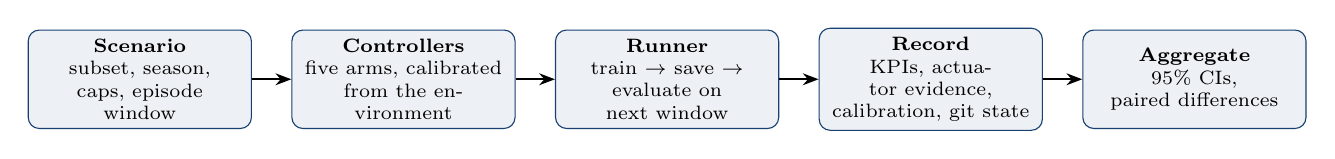
\begin{tikzpicture}[
  box/.style={draw=stemsblue, fill=stemsblue!8, rounded corners, align=center, minimum height=1.25cm, text width=2.6cm, font=\scriptsize},
  arr/.style={-{Stealth[length=2mm]}, thick}]
\node[box] (sc) {\textbf{Scenario}\\subset, season,\\caps, episode window};
\node[box, right=0.5cm of sc] (ct) {\textbf{Controllers}\\five arms, calibrated\\from the environment};
\node[box, right=0.5cm of ct] (rn) {\textbf{Runner}\\train $\rightarrow$ save $\rightarrow$\\evaluate on next window};
\node[box, right=0.5cm of rn] (js) {\textbf{Record}\\KPIs, actuator evidence,\\calibration, git state};
\node[box, right=0.5cm of js] (ag) {\textbf{Aggregate}\\95\% CIs,\\paired differences};
\draw[arr] (sc) -- (ct); \draw[arr] (ct) -- (rn); \draw[arr] (rn) -- (js); \draw[arr] (js) -- (ag);
\end{tikzpicture}}
\vspace{0.8em}
\begin{columns}[T]
\column{0.5\textwidth}
\begin{block}{Engineering}
\begin{itemize}
  \item Parallel and resumable; failures recorded, not raised.
  \item Runs whose actuators fail the check are excluded and counted.
\end{itemize}
\end{block}
\column{0.5\textwidth}
\begin{block}{Status}
\begin{itemize}
  \item 127 tests passing (library, harness and the new episode-window guard).
  \item First smoke grid exposed the autosizing defect; next: re-run with episode windows and fully equipped subsets.
\end{itemize}
\end{block}
\end{columns}
\end{frame}

% =====================================================================
\section{Heat pump standalone, Thermia and hygiene}
% =====================================================================

\begin{frame}{The heat-pump controller runs on its own}
\begin{columns}[T]
\column{0.5\textwidth}
\textbf{Isolation by device name}
\begin{align*}
\texttt{heatpump} &= [\,\text{heat pump}\,]\\
\texttt{thermal} &= [\,\text{hot water},\ \text{heat pump}\,]
\end{align*}
\begin{itemize}
  \item Non-controlled devices held at 0: for storage, exactly ``do nothing''.
  \item Battery barrier skipped when the battery is not controlled; power barriers stay on.
  \item Asking for a device the house lacks raises.
\end{itemize}
\column{0.5\textwidth}
\begin{block}{What standalone mode contains}
Encoder, policy, hot-water readiness $h_4$, CoP-aware power guard, dual set-point comfort. No battery, EV or neighbourhood coupling needed.
\end{block}
\begin{exampleblock}{Staged adoption}
E4 measured $h_4$ on a conventional reactive controller: an installation can adopt the \textbf{safety and anticipation layer first} and a learned policy later.
\end{exampleblock}
\end{columns}
\end{frame}

\begin{frame}{Integration with a commercial heat-pump platform (Thermia)}
\begin{columns}[T]
\column{0.5\textwidth}
\textbf{Signals needed}
\small
\begin{tabular}{@{}ll@{}}
\toprule
Outdoor temperature + forecast & hourly \\
Indoor temperature, set points & hourly \\
Tank temperature or state & hourly \\
Hot-water draw (past) & hourly \\
Electrical import, price & hourly \\
Rated power, tank size, efficiencies & once \\
\bottomrule
\end{tabular}
\column{0.5\textwidth}
\textbf{Steps}
\begin{enumerate}
  \item \textbf{Calibrate at commissioning}: read the installed unit's ratings (the lesson of E1 and E3).
  \item \textbf{Barrier at the edge}: analytic, no solver, no neighbourhood state, no connectivity dependence.
  \item \textbf{Forecaster learns on site}: no data leaves the house.
  \item \textbf{Policy optional} at first.
\end{enumerate}
\end{columns}
\vspace{0.4em}
\begin{alertblock}{Before any Nordic claim}
Heating-dominated climate; ground-source brine temperature instead of outdoor air in the CoP; inverter vs on-off control; hot-water heat pump with CoP penalty at 60\,$^\circ$C.
\end{alertblock}
\end{frame}

\begin{frame}{Legionella as a periodic deadline (proposed)}
\textbf{Thermia rule} (via Manal): at least once per week the tank reaches $60\,^\circ$C for a set duration $D$ (duration being confirmed).
\vspace{0.3em}

Energy-equivalent state for $60\,^\circ$C and a counter $c_t$ of hours since the last completed cycle, $W = 168$ h:
\[
s^{\text{leg}} = \frac{T^{\text{leg}} - T^{\text{cold}}}{T^{\max} - T^{\text{cold}}},
\qquad
\text{slack}^{\text{leg}}_t = (W - c_t) - \Big\lceil \frac{(s^{\text{leg}} - s_t)^+}{\rho} \Big\rceil - D
\]
Start the cycle when $\text{slack}^{\text{leg}}_t \le 0$; before that, the cycle may be moved to the cheapest or warmest feasible hours.
\vspace{0.3em}
\begin{columns}[T]
\column{0.5\textwidth}
\begin{block}{Why it fits}
Same object as $h_4$ and EVs: a required state, a deadline, a finite rate, plus a dwell time $D$.
\end{block}
\column{0.5\textwidth}
\begin{alertblock}{Open questions}
Cycle length; fixed or movable time; heat pump alone or with an electric backup; CityLearn tanks store energy, not temperature.
\end{alertblock}
\end{columns}
\end{frame}

\begin{frame}{Meeting with Manal: points to integrate}
\begin{columns}[T]
\column{0.5\textwidth}
\begin{block}{Discussed}
\begin{itemize}
  \item Test on different \textbf{consumer profiles}: residential and commercial.
  \item Add \textbf{hygiene} (anti-Legionella cycle).
  \item Report \textbf{as many KPIs as possible}.
  \item Test on \textbf{Thermia data} once the model is ready.
  \item Move the paper \textbf{beyond a benchmark study}.
\end{itemize}
\end{block}
\column{0.5\textwidth}
\begin{block}{How each maps onto the plan}
\begin{itemize}
  \item Profiles $\rightarrow$ another source of variation in the statistics.
  \item Hygiene $\rightarrow$ a new constraint, not a new mechanism.
  \item KPIs $\rightarrow$ extended KPI set (already implemented).
  \item Thermia $\rightarrow$ integration steps above.
  \item Framing $\rightarrow$ the research question on slide 3.
\end{itemize}
\end{block}
\end{columns}
\end{frame}

% =====================================================================
\section{Positioning in the literature}
% =====================================================================

\begin{frame}{RL for domestic hot water (papers shared by Manal)}
\scriptsize
\begin{tabularx}{\textwidth}{@{}>{\raggedright\arraybackslash}p{3.4cm}>{\raggedright\arraybackslash}X>{\raggedright\arraybackslash}p{4.1cm}@{}}
\toprule
Paper & Approach & Reported result \\
\midrule
Ali and Kazmi (2017), LNCS & Model-free RL, nZEBs, Utrecht (abstract not accessible) & minimise grid interaction of PV and hot water \\
De Somer et al.\ (2017), ISGT Europe & Model-based RL schedules hot-water buffer cycles; 6 real homes & self-consumption significantly up vs thermostat \\
Soares et al.\ (2020), Energy and Buildings & Model-based RL field test; heat-pump buffers and batteries & +14\% PV self-consumption, no discomfort \\
Heidari et al.\ (2021), J.\ Phys.\ Conf.\ Ser. & RL balancing energy, comfort and \textbf{hygiene}; measured use in one home, 8 weeks & 24.5\% energy saving, comfort and hygiene preserved \\
Langer and V\"olling (2022), Applied Energy & DDPG vs full-information MPC and rule-based; heat pump, PV, battery, storage & 75\% self-sufficiency, limited comfort violations \\
Amasyali et al.\ (2023), ORNL & DQN agents, electricity- or emission-focused, on a heat-pump water heater; several usage and marginal-emission profiles & 12--22\% less electricity; 18--37\% lower emissions \\
\bottomrule
\end{tabularx}
\vspace{0.4em}
\begin{block}{Gap (from the five abstracts available)}
Comfort and hygiene are objectives or soft penalties; none mentions guaranteed constraint satisfaction, a safety layer, or constraints shared across buildings. Heidari et al.\ also have two 2022 Applied Energy papers on hygiene, to be read before the Legionella design.
\end{block}
\end{frame}

\begin{frame}{Coordination, EVs and barrier functions}
\small
\begin{tabularx}{\textwidth}{@{}>{\raggedright\arraybackslash}p{4.1cm}>{\raggedright\arraybackslash}X@{}}
\toprule
Work & Relation to ours \\
\midrule
arXiv:2602.19223 (2026), CityLearn MARL benchmark & Decentralised training beats centralised; no analysis of constraint tightness. Our sweep offers an explanation: nothing binds. \\
arXiv:2605.01362 (2026), coordination architectures, Vermont & Hierarchical decomposition works best; explicitly no caps, EVs or deadlines. \\
arXiv:2607.00935 (2026), deadline-aware EV charging with transformer ageing & Soft deadlines and a marginal-cost urgency index (richer than EDF); four discrete scenarios, no capacity sweep. A rule to adopt and compare. \\
Input-constrained and backup CBFs (survey) & Our deadline barrier is a discrete-time, rate-limited instance; the contribution is the measured rate and the horizon rule, not a new theorem. \\
arXiv:2608.16335 (2026), ``readiness barrier functions'' & Multirotor actuator authority, different mathematics; name collision avoided. \\
\bottomrule
\end{tabularx}
\end{frame}

% =====================================================================
\section{Limitations and next steps}
% =====================================================================

\begin{frame}{Limitations we state openly}
\begin{columns}[T]
\column{0.5\textwidth}
\begin{itemize}
  \item One climate so far (cooling-dominated Texas).
  \item Prices and carbon borrowed from California; price forecasts exact.
  \item EV schedules synthetic.
  \item Seed spreads were zero (determinism), so no confidence intervals yet.
  \item Heat-pump-only converged result; joint run pending.
\end{itemize}
\column{0.5\textwidth}
\begin{itemize}
  \item Learned coordination not yet compared (training budget).
  \item Pre-heating results to be recomputed after the calendar and horizon fixes.
  \item Controllable share of load small when the battery is frozen.
  \item Indoor temperature from an LSTM surrogate.
  \item Tank model has no temperature (Legionella).
\end{itemize}
\end{columns}
\end{frame}

\begin{frame}{Next steps, in order}
\begin{enumerate}
  \item Fix the forecaster calendar and horizon defects and the tank-capacity fallback; recompute E4 and E5; regression-check.
  \item Re-run the smoke grid with episode windows and fully equipped subsets.
  \item Reference configuration: five-arm ablation with seeds, subsets and periods; 95\% CIs.
  \item Calibrated baselines: improved rules with Manal; perfect-forecast MPC.
  \item Cap sweep on the joint configuration and all arms.
  \item Heating-dominated scenario; Legionella as a periodic deadline.
  \item Quantitative EV experiment with competing devices; price-aware scheduling within the slack.
  \item Forecast-error robustness; then Thermia data.
\end{enumerate}
\end{frame}

\begin{frame}{Take-home messages}
\begin{enumerate}
  \item \textbf{Measure, do not assume}: one unchecked constant explained most violations; one unchecked convention broke the forecaster.
  \item \textbf{Match horizons to lead times}: the deficit collapses exactly where the measured fill time says.
  \item \textbf{One abstraction}: hot water, EVs and batteries are stores with deadlines.
  \item \textbf{Coupling changes the guarantee}: under a shared cap the safe set can be empty; detect it and degrade explicitly.
  \item \textbf{Coordination has a sweet spot}: worthless when slack, most valuable at intermediate caps.
  \item \textbf{Shield and learning interact}: a barrier that guarantees an objective removes the signal to learn it.
  \item \textbf{Test mechanisms where they can act}: slack caps and frozen devices hide everything.
\end{enumerate}
\vspace{0.6em}
\centering\Large Questions and discussion
\end{frame}

\end{document}
